% -*- coding: utf-8 -*-

\begin{chapter}{Волны в океане}\label{chap:16}
% \chapter{Ocean Waves} 
Глядя с берега на морскую поверхность, мы можем увидеть на ней волны. Если
присмотреться повнимательнее, станет очевидно, что волны представляют собой
неровности поверхности моря с высотой около метра, где под высотой понимается
расстояние по вертикали между нижней точкой некоторого углубления и 
%% trough еще и "подошва волны" (Мультитран)
расположенным рядом с ним гребнем волны. Длина волн, которую можно определить
как расстояние между явно выраженными гребнями, составляет около~$50$--$100\m$.
Наблюдая за волнением в течение нескольких минут, можно также заметить, что
и высота, и длина волн не являются постоянными. Высоты варьируют случайным
образом во времени и пространстве, а статистические свойства волн, такие как
средняя высота, вычисленная по выборке из нескольких сотен волн, меняются
ежесуточно. Эти хорошо заметные прибрежные волны имеют ветровую природу.
Так, иногда они возникают под воздействием
местных ветров, а иногда отдаленные штормы порождают волны, которые в конечном
итоге достигают берега. К примеру, волны, обрушивающиеся летним днем на
побережье Южной Калифорнии, могли перед этим преодолеть расстояние 
в~$10\,000\km$, дойдя туда от побережья Антарктиды, где они зародились в одном
из обширных штормов.
%
% Looking out to sea from the shore, we can see waves on the sea
% surface.  Looking carefully, we notice the waves are undulations of
% the sea surface with a height of around a meter, where height is the
% vertical distance between the bottom of a trough and the top of a
% nearby crest. The wavelength, which we might take to be the distance
% between prominent crests, is around 50-100 meters.  Watching the waves
% for a few minutes, we notice that wave height and wave length are not
% constant. The heights vary randomly in time and space, and the
% statistical properties of the waves, such as the mean height averaged
% for a few hundred waves, change from day to day. These prominent
% offshore waves are generated by wind. Sometimes the local wind
% generates the waves, other times distant storms generate waves which
% ultimately reach the coast. For example, waves breaking on the
% Southern California coast on a summer day may come from vast storms
% offshore of Antarctica 10,000 km away.

Благодаря более длительным наблюдениям, мы можем также отметить, что уровень
моря изменяется ежечасно. В течение суток этот уровень подымается и опускается
относительно некоторой выбранной на побережье точки примерно на метр. Такое
медленное изменение уровня моря происходит благодаря приливам~--- еще одной
разновидности волн на морской поверхности. Длина приливных волн\index{приливы} 
имеет порядок тысяч километров, а причиной их возникновения служат медленные
и крайне малые по величине изменения силы тяжести, возникающие благодаря
гравитационному взаимодействию движущихся относительно друг друга Земли,
Солнца\index{Солнце} и Луны\index{Луна}.
%
% If we watch closely for a long time, we notice that sea level changes
% from hour to hour. Over a period of a day, sea level increases and
% decreases relative to a point on the shore by about a meter. The slow
% rise and fall of sea level is due to the tides, another type of wave
% on the sea surface. Tides\index{tides} have wavelengths of thousands
% of kilometers, and they are generated by the slow, very small changes
% in gravity due to the motion of the sun\index{sun} and the
% moon\index{moon} relative to earth.

В этой главе мы рассмотрим способы описания количественных характеристик
поверхностных океанских волн, а в следующей~--- приливы и and waves along
coasts.
%
% In this chapter you will learn how to describe ocean-surface waves
% quantitatively. In the next chapter I will describe tides and waves along
% coasts.

\begin{section}{Линейная теория поверхностных океанских волн}\label{sec:LinWaves}
% \section{Linear Theory of Ocean Surface Waves}
\index{волны!линейная теория}Поверхностные волны в океане имеют существенно
нелинейную природу. Так, решение уравнений движения зависит от граничных 
условий на поверхности, но эти условия и есть те самые поверхностные волны,
картину которых нам требуется рассчитать. Как же можно выйти из этой ситуации?
%
% \index{waves!linear theory}Surface waves are inherently nonlinear: The
% solution of the equations of motion depends on the surface boundary
% conditions, but the surface boundary conditions are the waves we wish
% to calculate. How can we proceed?

Начнем с предположения, что амплитуда поверхностных волн бесконечно мала,
и поверхность практически представляет собой плоскость. Чтобы упростить
математические выкладки, мы можем также предположить, что поток двумерен,
а волны перемещаются в направлении оси абсцисс~$x$. Наконец, положим,
что силой Кориолиса и эффектами вязкости можно пренебречь.
Если же мы учтем и влияние суточного вращения Земли,
то наши теоретические построения охватят также волны Кельвина%
\index{волны!Кельвина}, которые обсуждались в разд.~\ref{sec:ElNino}.
%
% We begin by assuming that the amplitude of waves on the water surface is
% infinitely small so the surface is almost exactly a plane. To simplify the
% mathematics, we can also assume that the flow is 2-dimensional with waves
% traveling in the $x$-direction. We also assume that the Coriolis
% force and viscosity can be neglected. If we retain rotation, we get
% Kelvin\index{waves!Kelvin} waves discussed in \S 14.2.

С учетом этих предположений, превышение~$\zeta$ над морской поверхностью 
волны, движущейся в направлении оси~$x$, составит:
\begin{equation}
 \zeta = a \sin (k \, x - \omega \, t),
\end{equation}
где
\begin{eqnarray}
  \omega = 2 \pi f = \frac{2 \pi}{T}, & & k = \frac{2 \pi}{L},
\end{eqnarray}
причем $\omega$~--- циклическая частота волны размерностью рад/с,
а~$f$~--- частота в герцах, $k$~--- волновое число, 
$T$~--- период волны, а~$L$~--- её длина; при этом, согласно предположению,
$ka = O(0)$.
%
% With these assumptions, the sea-surface elevation $\zeta$ of a wave
% traveling in the $x$ direction is:
% \begin{equation}
% \zeta = a \sin (k \, x - \omega \, t)
% \end{equation}
% with
% \begin{eqnarray}
% \omega = 2 \pi f = \frac{2 \pi}{T}; & & k = \frac{2 \pi}{L}
% \end{eqnarray}
% where $\omega$ is wave frequency in radians per second, $f$ is the
% wave frequency in Hertz (Hz), $k$ is wave number, $T$ is wave period,
% $L$ is wave length, and where we assume, as stated above, that $ka =
% O(0)$.

\emph{Периодом волны}\index{волны!период|textbf}~$T$ называется время,
требуемое двум последовательным гребням волн или углублениям поверхности,
чтобы пройти через некоторую фиксированную точку пространства.
\emph{Длина волны}\index{волны!длина|textbf}~$L$~--- расстояние между двумя
последовательными гребнями волн или углублениями в заданный момент времени.
%
% The \textit{wave period}\index{waves!period|textbf} $T$ is the time it
% takes two successive wave crests or troughs to pass a fixed point. The
% \textit{wave length}\index{waves!length|textbf} $L$ is the distance
% between two successive wave crests or troughs at a fixed time.

\begin{paragraph}{Дисперсионное соотношение.}
% \paragraph{Dispersion Relation}
\index{waves!дисперсионное соотношение|textbf}%
\index{дисперсионное соотношение|textbf}Взаимосвязь циклической частоты~$\omega$ 
и волнового числа~$k$ определяется
\emph{дисперсионным соотношением} (Lamb, 1945 \S{228}):
\begin{equation}
 \omega ^{2} = g \, k \Tanh (k d),
\end{equation}
где $d$~--- глубина, а~$g$~--- ускорение силы тяжести.
%
% \index{waves!dispersion relation|textbf}\index{dispersion
% relation|textbf}Wave frequency $\omega$ is related to wave number $k$
% by the \textit{dispersion relation} (Lamb, 1945 \S{228}):
% \begin{equation}
% \omega ^{2} = g \, k \tanh (k d)
% \end{equation}
% where $d$ is the water depth and $g$ is the acceleration of gravity.

Два приближения особенно полезны на практике.
%
% Two approximations are especially useful.
\begin{enumerate}
\item \emph{Приближение глубокой воды} применимо в случае существенного
превышения глубиной~$d$ длины волны~$L$. При этом~$d \gg L$,
$kd \gg 1$, а~$\Tanh (kd) = 1$.
%
% \item \textit{Deep-water approximation} is valid if the water depth
% $d$ is much greater than the wave length $L$. In this case, $d \gg L$,
% $kd \gg 1$, and $\tanh (kd) = 1$.

\item \emph{Приближение мелкой воды} справедливо, когда глубина значительно
меньше длины волны. В этом случае $d \ll L$, $kd \ll 1$, а~$\Tanh (kd) = kd$.
%
% \item \textit{Shallow-water approximation} is valid if the water depth
% is much less than a wavelength. In this case, $d \ll L$, $kd \ll 1$,
% and $\tanh (kd) = kd$.
\end{enumerate}
Для этих двух предельных случаев соотношения глубины с длиной волны
дисперсионное соотношение принимает вид:
%
% For these two limits of water depth compared with wavelength the
% dispersion relation reduces to:
\begin{align}
  \omega ^2 &= g \, k & & \text{дисперсионное соотношение в глубокой воде,} \label{eq:16.4}\\
  d &> L/4, & &  \nonumber \\
   & & \nonumber \\
  \omega ^2 &= g \, k^{2} \, d & & \text{дисперсионное соотношение в мелкой воде,}\label{eq:16.5}\\
   d &< L/11. & & \nonumber
\end{align}
Приведенные ограничения на~$d/L$ обеспечивают выполнение дисперсионного 
соотношения с погрешностью, не превышающей~$10\%$. Поскольку многие 
характеристики волны могут быть измерены с погрешностью~$5$--$10\%$, 
предложенные приближения имеют практическую ценность при расчете 
характеристик волн. В дальнейшем мы рассмотрим способы вычисления 
этих характеристик в случае, когда волна распространяется 
от глубоких вод к мелким.
%
% The stated limits for $d/L$ give a dispersion relation accurate within
% 10\%.  Because many wave properties can be measured with accuracies of
% 5--10\%, the approximations are useful for calculating wave
% properties. Later we will learn to calculate wave properties as the
% waves propagate from deep to shallow water.
\end{paragraph}

\begin{paragraph}{Фазовая скорость.}
% \paragraph{Phase Velocity}
\index{волны!фазовая скорость}\index{фазовая скорость}Фазовой скоростью~$c$ 
называется скорость распространения некоторой фазы волны, например, скорость
распространения гребня волны. На временном промежутке, равном периоду~$T$,
гребень перемещается на расстояние, равное длине волны~$L$, а фазовая 
скорость, соответственно: $c=L/T= \omega /k$. 
Таким образом, определение фазовой скорости принимает вид:
   \begin{equation}
      c \equiv \frac {\omega}{k}.
   \end{equation}
Направление распространения волны перпендикулярно ее гребню и совпадает
с положительным направлением оси абсцисс~$x$. 
%
% \index{waves!phase velocity}\index{phase velocity}The phase velocity
% $c$ is the speed at which a particular phase of the wave propagates,
% for example, the speed of propagation of the wave crest. In one wave
% period $T$ the crest advances one wave length $L$ and the phase speed
% is $c=L/T= \omega /k$. Thus, the definition of phase speed is:
%    \begin{equation}
%       c \equiv \frac {\omega}{k}
%    \end{equation}
% The direction of propagation is perpendicular to the wave crest and toward the
% positive $x$ direction. 

Применив приближения мелкой и глубокой воды для дисперсионного соотношения, 
получаем:
  \begin{align}
   c &= \sqrt{\frac{g}{k}} = \frac{g}{\omega} & & \text{фазовая скорость в глубокой воде,} \label{eq:16.7}\\
   & &  & \nonumber \\
   c &=\sqrt{g\,d} & & \text{фазовая скорость в мелкой воде.}\label{eq:16.8}
  \end{align}
Погрешность приближения составляет около~$5\%$ для пределов, 
установленных в (\ref{eq:16.4}) и~(\ref{eq:16.5}).
%
% The deep- and shallow-water approximations for the dispersion
% relation give:
%   \begin{align}
%    c &= \sqrt{\frac{g}{k}} = \frac{g}{\omega} & & \text{ Deep-water phase
% velocity} \\
%    & &  & \nonumber \\
%    c &=\sqrt{g\,d} & & \text{ Shallow-water phase velocity}
%   \end{align}
% The approximations are accurate to about 5\% for limits stated in (16.4, 16.5).

В глубокой воде фазовая скорость зависит от длины волны либо ее частоты. 
Более длинные волны движутся быстрее. Это явление называется \emph{дисперсией},
а про волны в глубокой воде говорят, что они диспергируют (или разбегаются). 
В мелкой воде, напротив, фазовая скорость от характеристик волны не зависит,
а определяется исключительно глубиной. Таким образом, волны в мелкой
воде не подвержены дисперсии.
%
% In deep water, the phase speed depends on wave length or wave
% frequency. Longer waves travel faster. Thus, deep-water waves are said
% to be dispersive. In shallow water, the phase speed is independent of
% the wave; it depends only on the depth of the water. Shallow-water
% waves are non-dispersive.
\end{paragraph}

\begin{paragraph}{Групповая скорость.}
% \paragraph{Group Velocity}
\index{волны!групповая скорость}\index{групповая скорость}Понятие групповой
скорости~$c_{g}$ лежит в основе понимания механизма распространения 
линейных и нелинейных волн. Прежде всего, это скорость, с которой группа волн
движется через океан. Более важно, что это также и скорость распространения
энергии волн.
Уизем дает в работе (Whitham, 1974, \S~1.3 и~\S~11.6) ясное определение этого
понятия и выводит фундаментальное уравнение~(\ref{eq:16.9}).
%
% \index{waves!group velocity}\index{group velocity}The concept of group
% velocity $c_{g}$ is fundamental for understanding the propagation of
% linear and nonlinear waves. First, it is the velocity at which a group
% of waves travels across the ocean. More importantly, it is also the
% propagation velocity of wave energy. Whitham (1974, \S 1.3 and \S
% 11.6) gives a clear derivation of the concept and the fundamental
% equation (16.9).

Определение групповой скорости в двумерном случае таково:
\begin{equation}\label{eq:16.9}
  c_{g} \equiv \frac {\partial \omega }{\partial k}.
\end{equation}
Используя приближенные дисперсионные соотношения, получаем:
 \begin{align}
 c_{g} &= \frac{g}{2\omega} = \frac{c}{2} & &   \text{групповая скорость в глубокой воде,}\label{eq:16.10} \\
  & & & \nonumber \\
 c_{g} &= \sqrt{g\,d} \, = c & &   \text{групповая скорость в мелкой воде.}\label{eq:16.11}
 \end{align}
Направление распространения поверхностных волн в океане перпендикулярно
гребням волн и совпадает с положительным направлением оси абсцисс~$x$. 
В более общем случае волн иных типов, таких как волны 
Кельвина\index{волны!Кельвина} и Россби\index{волны!Россби}, которые мы
упоминали в разд.~\ref{sec:ElNino}, направление вектора групповой скорости 
не обязательно будет перпендикулярно гребням волн.
%
% The definition of group velocity in two dimensions is:
% \begin{equation}
% c_{g} \equiv \frac {\partial \omega }{\partial k}
% \end{equation}
% Using the approximations for the dispersion relation:
%  \begin{align}
%  c_{g} &= \frac{g}{2\omega} = \frac{c}{2} & &   \text{ Deep-water group velocity} \\
%   & & & \nonumber \\
%  c_{g} &= \sqrt{g\,d} \, = c & &   \text{ Shallow-water group velocity}
%  \end{align}
% For ocean-surface waves, the direction of propagation is perpendicular
% to the wave crests in the positive $x$ direction. In the more general
% case of other types of waves, such as Kelvin\index{waves!Kelvin} and
% Rossby\index{waves!Rossby} waves that we met in \S14.2, the group
% velocity is not necessarily in the direction perpendicular to wave
% crests.

Отметим, что группа волн в глубокой воде перемещается с скоростью,
равной половине фазовой скорости волн, составляющих эту группу. В чем причина
такого явления? Если бы мы могли присмотреться с небольшого расстояния
к группе волн, пересекающих океан, мы могли бы увидеть гребни волн, 
возникающих позади волнового цуга, перемещающихся через него и исчезающих
на его переднем краю. Каждый гребень волны движется со скоростью,
в два раза большей скорости группы.
%
% Notice that a group of deep-water waves moves at half the phase speed
% of the waves making up the group. How can this happen? If we could
% watch closely a group of waves crossing the sea, we would see waves
% crests appear at the back of the wave train, move through the train,
% and disappear at the leading edge of the group. Each wave crest moves
% at twice the speed of the group.

Возникает вопрос: будут ли реальные океанские волны перемещаться группами,
подчиняясь дисперсионному соотношению? Ответ на него положителен. Уолтер Манк
и его коллеги провели в 1960-х замечательную серию экспериментов, в ходе
которых было установлено, что волны, распространяющиеся в океане на огромные
расстояния, подвержены дисперсии, которая, в свою очередь, может 
использоваться для обнаружения штормов (Munk et al., 1963). 
Была организована регистрация волн на протяжении многих суток при помощи 
трех измерителей давления, установленных у побережья о-ва~Сан-Клементе, 
расположенного в 60~милях
%% каких: морских или сухопутных
к западу от Сан-Диего (Калифорния). По данным каждых суток наблюдений
вычислялись волновые спектры. (Понятие спектров будет рассматриваться далее.)
Затем по этим спектрам удалось определить амплитуды и частоты
низкочастотных волн, а также направление перемещения волн.
%% направление волн в целом или тех же самых, низкочастотных?
%% если тех же, можно второе упоминание волн заменить на "их".
Наконец, были построены графики волновой энергии, нанесенные на 
частотно-временную диаграмму (рис.~\ref{fig:dispersedwaves}).
%
% Do real ocean waves move in groups governed by the dispersion
% relation? Yes.  Walter Munk and colleagues (1963) in a remarkable
% series of experiments in the 1960s showed that ocean waves propagating
% over great distances are dispersive, and that the dispersion could be
% used to track storms. They recorded waves for many days using an array
% of three pressure gauges just offshore of San Clemente Island, 60
% miles due west of San Diego, California. Wave spectra were calculated
% for each day's data. (The concept of a spectra is discussed below.)
% From the spectra, the amplitudes and frequencies of the low-frequency
% waves and the propagation direction of the waves were
% calculated. Finally, they plotted contours of wave energy on a
% frequency-time diagram (figure 16.1).

Чтобы понять изображенное на этом рисунке, представим себе удаленный шторм,
порождающий волны различных частот. Волны с самой низкой частотой
(наименьшее значение параметра~$\omega$) распространяются быстрее 
других~(\ref{eq:16.11}), так что они прибывают к месту наблюдений скорее,
чем волны с б\'{о}льшими частотами. Чем больше расстояние до шторма,
тем длительнее задержка между приходом волн различных частот.
Пиковые значения высокой энергии волн, которые можно видеть на рисунке,
порождаются отдельными штормами. The slope of the ridge соответствует
расстоянию~$\Delta$ до шторма в градусах дуги большого круга; 
кроме этого, информация о фазе, полученная группировкой измерителей,
позволяет определить angle to the storm $\theta$. 
По этим двум углам возможно восстановить расположение шторма относительно
о-ва~Сан-Клементе. Так, волны, зарегистрированные в период с~15 по~18~сентября,
образуют пик, соответствующий шторму, прошедшему на угловом 
расстоянии~$\degrees{115}$ под углом~$\degrees{205}$, то есть,
южнее Новой Зеландии вблизи Антарктиды.
%
% To understand the figure, consider a distant storm that produces waves
% of many frequencies. The lowest-frequency waves (smallest $\omega$)
% travel the fastest (16.11), and they arrive before other,
% higher-frequency waves. The further away the storm, the longer the
% delay between arrivals of waves of different frequencies. The ridges
% of high wave energy seen in the figure are produced by individual
% storms. The slope of the ridge gives the distance to the storm in
% degrees $\Delta$ along a great circle; and the phase information from
% the array gives the angle to the storm $\theta$. The two angles give
% the storm's location relative to San Clemente. Thus waves arriving
% from 15 to 18 September produce a ridge indicating the storm was
% 115\degrees\ away at an angle of 205\degrees\ which is south of new
% Zealand near Antarctica.

Было проведено сравнение местоположения штормов, породивших волны, 
зарегистрированные за период с~июня по~октябрь 1959~г., с данными о штормах,
нанесенными на метеорологические карты. В большинстве случаев достигнуто
хорошее согласование. 
%
% The locations of the storms producing the waves recorded from June
% through October 1959 were compared with the location of storms plotted
% on weather maps and in most cases the two agreed well.
\end{paragraph}

\begin{figure}[t!]
\makebox[121mm][c]{\includegraphics{pics/dispersedwaves}}
\caption{Изолинии энергии волн, нанесенные на частотно-временную диаграмму,
которые были вычислены по спектрам, полученным по данным измерителей давления,
установленных у побережья Южной Калифорнии. Пики высокой энергии волн
указывают моменты прибытия диспергированных волновых цугов, порожденных 
удаленными штормами. The slope of the ridge обратно пропорционален 
расстоянию до шторма. Величина~$\Delta$~--- расстояние в градусах, 
$\theta$~--- направление прибытия волн к побережью Калифорнии. 
(Munk et al., 1963).}
\label{fig:dispersedwaves}
\end{figure}
%
% \begin{figure}[t!]
% \makebox[121mm][c]{\includegraphics{dispersedwaves}}
% \footnotesize
% Figure 16.1 Contours \rule{0mm}{4ex}of wave energy on a frequency-time
% plot calculated from spectra of waves measured by pressure gauges
% offshore of southern California. The ridges of high wave energy show
% the arrival of dispersed wave trains from distant storms. The slope of
% the ridge is inversely proportional to distance to the storm.
% $\Delta$ is distance in degrees, $\theta$ is direction of arrival of
% waves at California. After Munk et al. (1963).
% \label{fig:dispersedwaves}
% \vspace{-3ex}
% \end{figure}

\begin{paragraph}{Энергия волн.}
% \paragraph{Wave Energy}
\index{волны!энергия}Энергия волн~$E$, измеряемая в джоулях на квадратный
метр, связана с дисперсией%
\remark{В данном случае этот термин обозначает характеристику случайной
величины, а не явление разбегания волн.}
смещения морской поверхности~$\zeta$ следующим
отношением:
 \begin{equation}\label{eq:16.12}
 E = \rho _{w} g \, \left< \zeta ^{2} \right>,
 \end{equation}
где~$\rho _{w}$~--- плотность воды, $g$~--- ускорение силы тяжести, 
а угловые скобки обозначают осреднение по времени либо пространству.
%
% \index{waves!energy}Wave energy $E$ in Joules per square meter is
% related to the variance of sea-surface displacement $\zeta$ by:
%  \begin{equation}
%  E = \rho _{w} g \, \left< \zeta ^{2} \right>
%  \end{equation}
% where $\rho _{w}$ is water density, $g$ is gravity, and the brackets
% denote a time or space average.
\end{paragraph}

\begin{figure}[h!]
\vspace{1ex}
\begin{center}
\makebox[121mm][c]{\includegraphics{pics/waveheight}}
\end{center}
\caption{График амплитуды волн, измеренной на коротком промежутке времени
wave buoy, установленным в Северной Атлантике.}
\label{fig:waveheight}
\end{figure}
%
% \begin{figure}[h!]
% \vspace{1ex}
% \makebox[121mm][c]{\includegraphics{waveheight}}
% \centering
% \footnotesize
% Figure 16.2 A short record \rule{0mm}{3ex}of wave amplitude measured\\
% by a wave buoy in the north Atlantic.
%
% \label{fig:waveheight}
% \vspace{-1ex}
% \end{figure}

\begin{paragraph}{Значимая высота волн.}
% \paragraph{Significant Wave Height}
\index{волны!значимая высота}Что подразумевается под высотой волны? 
Если мы посмотрим на море, находящееся под воздействием ветра, мы увидим
волны различной высоты. Некоторые из них гораздо выше большинства,
некоторые же существенно меньше (рис.~\ref{fig:waveheight}). 
На практике часто пользуются такой характеристикой, как высота наивысшей
трети волн, обозначаемой как~$H_{1/3}$. Эта высота рассчитывается 
следующим образом: в течение нескольких минут измеряется высота волн,
среди них выбираются, к примеру, 120 гребней, высота которых фиксируется.
Далее среди них выбираются высоты 40~наибольших волн, для которых вычисляется
среднее, которое и принято называть характеристикой~$H_{1/3}$ данной 
совокупности наблюдений.
%
% \index{waves!significant height}What do we mean by wave height? If we
% look at a wind-driven sea, we see waves of various heights. Some are
% much larger than most, others are much smaller (figure 16.2). A
% practical definition that is often used is the height of the highest
% 1/3 of the waves, $H_{1/3}$. The height is computed as follows:
% measure wave height for a few minutes, pick out say 120 wave crests
% and record their heights. Pick the 40 largest waves and calculate the
% average height of the 40 values. This is $H_{1/3}$ for the wave
% record.
% %The quantity $H_{1/3}$ was chosen because it
% %corresponds closely to wave height estimated by a trained observer looking at the
% %sea.

Понятие значимой высоты волн было предложено во время Второй мировой войны
в рамках проекта по прогнозированию высот и периодичности океанских волн.
Wiegel сообщает (Wiegel, 1964: p.  198), что работы Института океанографии
им. Скриппса показали следующее:
%
% The concept of significant wave height was developed during the World
% War II as part of a project to forecast ocean wave heights and
% periods. Wiegel (1964: p.  198) reports that work at the Scripps
% Institution of Oceanography showed
\begin{quote}
\ldots{} высота волн, полученная по оценкам наблюдателей, соответствует 
средней высоте наибольших 20--40\% волн\ldots{} 
Первоначально понятие значимой высоты волн было сопоставлено со средним 
значением этих наблюдений, или же наивысшими 30\%~волн, но оно в дальнейшем
эволюционировало и превратилось в наивысшую треть волн (и получило 
обозначение~$H_S$ или~$H_{1/3}$).
%
% \ldots wave height estimated by observers corresponds to the average
% of the highest 20 to 40 per cent of waves\ldots Originally, the term
% significant wave height was attached to the average of these
% observations, the highest 30 per cent of the waves, but has evolved to
% become the average of the highest one-third of the waves, (designated
% $H_S$ or $H_{1/3}$)
\end{quote}

В дальнейшем для вычисления значимой высоты волн стали использовать данные
измерений смещения морской поверхности под действием волн. Если в океане
зафиксирован узкий диапазон частот волн, величина~$H_{1/3}$ взаимосвязана
со среднеквадратичным отклонением смещения морской поверхности
(NAS, 1963: 22; Hoffman and Karst, 1975):
\begin{equation}
 H_{1/3} = 4 \left< \zeta ^{2}\right>^{1/2},
\end{equation}
где~$ \left< \zeta ^{2}\right>^{1/2}$~--- среднеквадратичное отклонение
смещения морской поверхности. Это соотношение значительно более полезно
на практике и в данный момент является общепринятым способом вычисления
высоты волн по данным измерений.
%
% More recently, significant wave height is calculated from measured
% wave displacement. If the sea contains a narrow range of wave
% frequencies, $H_{1/3}$ is related to the standard deviation of
% sea-surface displacement (\textsc{nas} , 1963: 22; Hoffman and Karst,
% 1975)
% \begin{equation}
% H_{1/3} = 4 \left< \zeta ^{2}\right>^{1/2}
% \end{equation}
% where $ \left< \zeta ^{2}\right>^{1/2}$ is the standard deviation of
% surface displacement. This relationship is much more useful, and it is
% now the accepted way to calculate wave height from wave measurements.
\end{paragraph}
\end{section}

\begin{section}{Нелинейные волны}
% \section{Nonlinear waves}
\index{волны!нелинейные}Нами были получены свойства поверхностных океанских 
волн в предположении, что их амплитуда бесконечно мала: $ka = O(0)$. 
Если же $ka \ll 1$, но не может считаться бесконечно малой, характеристики
волны могут быть выражены в виде степенного ряда по~$ka$ (Stokes, 1847). 
Стокс рассчитал свойства волны конечной амплитуды и обнаружил, что
\begin{equation}\label{eq:16.14}
 \zeta = a \cos(kx - \omega t) + \frac{1}{2} k a^{2}\cos 2(kx-\omega t) 
         + \frac{3}{8} k^{2} a^{3} \cos 3(k x - \omega t) + \ldots
\end{equation}
Фазы компонент разложения~$\zeta$ в ряд Фурье (\ref{eq:16.14}) таковы, 
что нелинейные волны имеют более острые гребни и пологие впадины.
Максимальная амплитуда волны, найденная Стоксом, $a_{max} = 0.07 L$ 
($ ka = 0.44$). Такие крутые волны в глубокой воде были названы волнами
Стокса (см. также (Lamb, 1945), \S~250).
%
% \index{waves!nonlinear}We derived the properties of an ocean surface
% wave assuming the wave amplitude was infinitely small $ka = O(0)$. If
% $ka \ll 1$ but not infinitely small, the wave properties can be
% expanded in a power series of $ka$ (Stokes, 1847). He calculated the
% properties of a wave of finite amplitude and found:
% \begin{equation}
% \zeta = a \cos(kx - \omega t) + \frac{1}{2} k a^{2}\cos 2(kx-\omega t) +
% \frac{3}{8} k^{2} a^{3} \cos 3(k x - \omega t) + \cdots
% \end{equation}
% The phases of the components for the Fourier series expansion of
% $\zeta$ in (16.14) are such that non-linear waves have sharpened
% crests and flattened troughs. The maximum amplitude of the Stokes wave
% is $a_{max} = 0.07 L$ ($ ka = 0.44$). Such steep waves in deep water
% are called Stokes waves (See also Lamb, 1945, \S 250).

Развитие теории нелинейных волн протекало медленно до тех пор, пока
Хассельманн (Hasselmann 1961, 1963a, 1963b, 1966), используя методы
физики высоких энергий, не разработал 
to 6th order теорию взаимодействия трех и более волн на морской поверхности.
В его работах, а также Филлипсом (Phillips, 1960), 
и Лонге-Хиггинсом совместно с Филлипсом (Longuet-Higgins and Phillips, 1962) 
было показано, что $n$~свободных волн на морской поверхности могут 
взаимодействовать, образуя в результате еще одну свободную волну только тогда,
когда суммы частот и волновых чисел взаимодействующих волн равны нулю:
\begin{subequations}\label{eq:16.15}
\begin{eqnarray}
 & \omega _{1} \pm \omega _{2} \pm \omega _{3} \pm \cdots \omega _{n}  = 0, & \\
 & \mbfk_{1} \pm  \mbfk_{2} \pm  \mbfk_{3} \pm \cdots \mbfk_{n} =  0,  & \\
 & \omega_{i}^{2} = g \, k_{i}, &
\end{eqnarray}
\end{subequations}
где волны могут перемещаться в любом направлении, а $\mbfk_{i}$~--- вектор
волновых чисел, задающий длину волны и направление ее распространения.
Соотношения~(\ref{eq:16.15}) являются общими требованиями ко всем 
взаимодействующим волнам. Наименьшее количество волн, которые в состоянии
удовлетворить условиям~(\ref{eq:16.15})~--- три волны, которые во 
взаимодействии порождают четвертую. Это взаимодействие слабо; волны должны
взаимодействовать на протяжении сотен длин волн и периодов, чтобы
в итоге породить четвертую волну сравнимой амплитуды. Волны Стокса не
соответствуют критериям~(\ref{eq:16.15}), а их компоненты не являются
свободными волнами; более высокочастотные гармоники связаны с первичной волной.
%
% Knowledge of non-linear waves came slowly until Hasselmann (1961,
% 1963a, 1963b, 1966), using the tools of high-energy particle physics,
% worked out to 6th order the interactions of three or more waves on the
% sea surface. He, Phillips (1960), and Longuet-Higgins and Phillips
% (1962) showed that $n$ free waves on the sea surface can interact to
% produce another free wave only if the frequencies and wave numbers of
% the interacting waves sum to zero:
% \begin{subequations}
% \begin{eqnarray}
%  & \omega _{1} \pm \omega _{2} \pm \omega _{3} \pm \cdots \omega _{n}  = 0
% & \\
%  & \mathbf{k_{1}} \pm  \mathbf{k_{2}} \pm  \mathbf{k_{3}} \pm \cdots
% \mathbf{k_{n}} =  0  &
% \\
%  & \omega_{i}^{2} = g \, k_{i} &
% \end{eqnarray}
% \end{subequations}
% where we allow waves to travel in any direction, and $\mathbf{k_{i}}$
% is the vector wave number giving wave length and direction. (16.15)
% are general requirements for any interacting waves. The fewest number
% of waves that meet the conditions of (16.15) are three waves which
% interact to produce a fourth. The interaction is weak; waves must
% interact for hundreds of wave lengths and periods to produce a fourth
% wave with amplitude comparable to the interacting waves. The Stokes
% wave does not meet the criteria of (16.15) and the wave components are
% not free waves; the higher harmonics are bound to the primary wave.

\begin{paragraph}{Wave Momentum.}
% \paragraph{Wave Momentum}
\index{waves!momentum}Понятие wave momentum послужило причиной существенной
путаницы (McIntyre, 1981). В целом, волны не обладают 
momentum, a mass flux, but they do have a momentum flux. 
Это справедливо и для поверхностных океанских волн.
Ursell показал, что зыбь в океане на поверхности вращающейся 
Земли не вызывает переноса массы\index{перенос!волновой} (Ursell, 1950).  
Его доказательство, на первый взгляд, противоречит принятому в учебниках
изложению свойств крутых нелинейных волн, таких как волны Стокса. Частицы
воды в волнах Стокса движутся практически по окружности, но траектории все
же не замыкаются, так что частицы медленно перемещаются в направлении
распространения волны. Таким образом, имеет место перенос массы, который
получил название дрейф Стокса. Однако, перенос массы в некотором направлении
у поверхности уравновешивается переносом в противоположном направлении,
происходящим на глубине, так что эффективный перенос массы будет нулевым.
%
% \index{waves!momentum}The concept of wave momentum has caused
% considerable confusion (McIntyre, 1981). In general, waves do not have
% momentum, a mass flux, but they do have a momentum flux. This is true
% for waves on the sea surface. Ursell (1950) showed that ocean swell on
% a rotating earth has no mass transport\index{transport!by waves}.  His
% proof seems to contradict the usual textbook discussions of steep,
% non-linear waves such as Stokes waves. Water particles in a Stokes
% wave move along paths that are nearly circular, but the paths fail to
% close, and the particles move slowly in the direction of wave
% propagation. This is a mass transport, and the phenomena is called
% Stokes drift. But the forward transport near the surface is balanced
% by an equal transport in the opposite direction at depth, and there is
% no net mass flux.
\end{paragraph}
\end{section}

\begin{section}{Волны и понятие волнового спектра}
% \section{Waves and the Concept of a Wave Spectrum}
%
\index{волны!спектры!понятие}Глядя на морскую поверхность, мы можем 
заметить, что форма волн не является синусоидой. Напротив, общая картина
волнения складывается из волн с различными длинами и периодами, распределение
которых случайно. Каким же образом можно построить описание подобной 
поверхности? К сожалению, это не слишком просто. Однако, мы можем, применив
некоторые упрощения, получить требуемое с достаточно высоким приближением
к реальности. На основе этих упрощений и было сформулировано понятие спектра
океанских волн. Спектр предоставляет нам распределение энергии по
различным частотам или длинам поверхностных океанских волн.
%
% \index{waves!spectra!concept}If we look out to sea, we notice that
% waves on the sea surface are not sinusoids. The surface appears to be
% composed of random waves of various lengths and periods. How can we
% describe this surface? The answer is, Not very easily. We can however,
% with some simplifications, come close to describing the surface. The
% simplifications lead to the concept of the spectrum of ocean
% waves. The spectrum gives the distribution of wave energy among
% different wave frequencies or wave lengths on the sea surface.

Основы теории спектров были заложены работами Жана Батиста Жозефа Фурье
(1768--1830), который показал, что практически любая функция вида~$\zeta(t)$ 
(или~$\zeta (x)$, если кто-то предпочитает такие обозначения), 
на интервале~$-T/2 \le t \le T/2$ может быть представлена в виде суммы
бесконечного ряда синусоид и косинусоид с кратными частотами:
\begin{equation}\label{eq:16.16}
  \zeta (t) = \frac{a_0}{2} + \sum_{n=1}^{\infty} (a_n \cos 2\pi nft + b_n \sin 2\pi nft),
\end{equation}
где
\begin{subequations}\label{eq:16.17}
\begin{align}
 a_n &= \frac{2}{T} \int_{-T/2}^{T/2} \zeta (t) \cos 2\pi nft \, dt, 
          \qquad (n=0,1,2,\ldots) \\
 b_n &= \frac{2}{T} \int_{-T/2}^{T/2} \zeta (t) \sin 2\pi nft \, dt, 
          \qquad (n=0,1,2,\ldots)
\end{align}
\end{subequations}
где~$f = 1/ T$~--- основная частота, и~$nf$~--- её гармоники. 
Такая форма представления~$\zeta (t)$ называется
\emph{рядом Фурье}\index{волны!ряды Фурье|textbf}\index{ряды Фурье|textbf} 
(Bracewell, 1986: 204; Whittaker and Watson, 1963: \S 9.1). 
Отметим, что $a_0$ равняется среднему значению~$\zeta (t)$ на заданном 
интервале.
%
% The concept of a spectrum is based on work by Joseph Fourier
% (1768--1830), who showed that almost any function $\zeta (t)$ (or
% $\zeta (x)$ if you like), can be represented over the interval $-T/2
% \le t \le T/2$ as the sum of an infinite series of sine and cosine
% functions with harmonic wave frequencies:
% \begin{equation}
% \zeta (t) = \frac{a_0}{2} + \sum_{n=1}^{\infty} (a_n \cos 2\pi nft + b_n \sin
% 2\pi nft)
% \end{equation}
% where
% \begin{subequations}
% \begin{align}
% a_n &= \frac{2}{T} \int_{-T/2}^{T/2} \zeta (t) \cos 2\pi nft \, dt, \qquad
% (n=0,1,2,\ldots) \\
% b_n &= \frac{2}{T} \int_{-T/2}^{T/2} \zeta (t) \sin 2\pi nft \, dt, \qquad
% (n=0,1,2,\ldots)
% \end{align}
% \end{subequations}
% $f = 1/ T$ is the fundamental frequency, and $nf$ are harmonics of the
% fundamental frequency. This form of $\zeta (t)$ is called a
% \textit{Fourier series}\index{waves!Fourier
% series|textbf}\index{Fourier series|textbf} (Bracewell, 1986: 204;
% Whittaker and Watson, 1963: \S 9.1). Notice that $a_0$ is the mean
% value of $\zeta (t)$ over the interval.

Чтобы упростить уравнения~(\ref{eq:16.16}) и~(\ref{eq:16.17}), можно 
%% в оригинале: (16.18 and 16.19)
воспользоваться соотношением
\begin{equation}
 \exp (2\pi inft) = \cos (2\pi nft) + i \sin (2\pi nft),
\end{equation}
где~$i = \sqrt{-1}$. При этом уравнения~(\ref{eq:16.16}) и~(\ref{eq:16.17}) 
%% в оригинале: (16.18 and 16.19)
принимают вид:
\begin{equation}\label{eq:16.19}
 \zeta (t) = \sum_{n=-\infty}^{\infty} Z_n \exp ^{i2\pi nft},
\end{equation}
где
\begin{equation}\label{eq:16.20}
  Z_n = \frac{1}{T} \int_{-T/2}^{T/2} \zeta (t) \exp ^{-i2\pi nft} \, dt, 
   \qquad (n=0,1,2,\ldots)
\end{equation}
называется \emph{преобразованием Фурье}%
\index{волны!преобразование Фурье|textbf}\index{преобразование Фурье|textbf} 
функции~$\zeta (t)$.
%
% Equations (16.18 and 16.19) can be simplified using
% \begin{equation}
% \exp (2\pi inft) = \cos (2\pi nft) + i \sin (2\pi nft)
% \end{equation}
% where $i = \sqrt{-1}$. Equations (16.18 and 16.19) then become:
% \begin{equation}
% \zeta (t) = \sum_{n=-\infty}^{\infty} Z_n \exp ^{i2\pi nft}
% \end{equation}
% where
% \begin{equation}
% Z_n = \frac{1}{T} \int_{-T/2}^{T/2} \zeta (t) \exp ^{-i2\pi nft} \, dt, \qquad
% (n=0,1,2,\ldots)
% \end{equation}
% $Z_n$ is called the \textit{Fourier transform}\index{waves!Fourier
% transform|textbf} \index{Fourier transform|textbf} of $\zeta (t)$.

Спектр~$S(f)$ функции~$\zeta (t)$ определяется как
\begin{equation}
 S(nf) = Z_n Z^*_n,
\end{equation}
где~$Z^*$~--- число, комплексно сопряженное с~$Z$. Мы будем использовать
такую форму записи рядов Фурье и спектров при описании процесса получения
волновых спектров океана.
%
% The spectrum $S(f)$ of $\zeta (t)$ is:
% \begin{equation}
% S(nf) = Z_n Z^*_n
% \end{equation}
% where $Z^*$ is the complex conjugate of $Z$. We will use these forms
% for the Fourier series and spectra when we describing the computation
% of ocean wave spectra.

Понятие рядов Фурье может быть обобщено на случай поверхностей 
вида~$\zeta (x,y)$.
Таким образом, любая поверхность представима в виде суммы
бесконечного ряда синусоид и косинусоид, ориентированных во всех возможных
направлениях.
%
% We can expand the idea of a Fourier series to include series that
% represent surfaces $\zeta (x,y)$ using similar techniques. Thus, any
% surface can be represented as an infinite series of sine and cosine
% functions oriented in all possible directions.

Применим изложенные идеи к морской поверхности. Предположим, что в некий
момент времени состояние этой поверхности было зафиксировано. Далее,
используя разложение Фурье, мы можем представить эту поверхность в виде
бесконечного ряда синусоид и косинусоид с различными волновыми числами,
ориентированных во всех возможных направлениях. Если же мы позволим
поверхности меняться во времени, она может быть также представлена в виде
бесконечного ряда синусоид и косинусоид с различными длинами волн, 
перемещающихся в различных направлениях. Поскольку длины волн и частоты
связаны дисперсионным соотношением, морская поверхность также может быть
представлена в виде суммы бесконечного количества синусоид и косинусоид
различных частот, перемещающихся во всех возможных направлениях.
%
% Now, let's apply these ideas to the sea surface. Suppose for a moment
% that the sea surface were frozen in time. Using the Fourier expansion,
% the frozen surface can be represented as an infinite series of sine
% and cosine functions of different wave numbers oriented in all
% possible directions. If we unfreeze the surface and let it move, we
% can represent the sea surface as an infinite series of sine and cosine
% functions of different wave lengths moving in all directions. Because
% wave lengths and wave frequencies are related through the dispersion
% relation, we can also represent the sea surface as an infinite sum of
% sine and cosine functions of different frequencies moving in all
% directions.

Отметим, что в приведенном выше обсуждении рядов Фурье мы полагали, что
коэффициенты~$a_n$, $b_n$ и~$Z_n$ постоянны. При временных масштабах около
одного часа и расстояниях порядка десятков километров характеристики 
поверхностных волн достаточно стабильны, чтобы считать это допущение верным.
Более того, нелинейные взаимодействия между волнами крайне слабы. 
Следовательно, локальное состояние морской поверхности может быть выражено
линейной суперпозицией реальных волн синусоидальной формы с различными длинами
волн, частотами и фазами, распространяющихся во множестве различных 
направлений. Ряды Фурье оказываются не только удобным математическим 
формализмом, it states that the sea surface is really, truly composed
of sine waves, каждая из которых подчиняется уравнениям, приведенным в
разд.~\ref{sec:LinWaves}.
%
% Note in our discussion of Fourier series that we assume the
% coefficients $(a_n, b_n, Z_n)$ are constant. For times of perhaps an
% hour, and distances of perhaps tens of kilometers, the waves on the
% sea surface are sufficiently fixed that the assumption is
% true. Furthermore, non-linear interactions among waves are very
% weak. Therefore, we can represent a local sea surface by a linear
% superposition of real, sine waves having many different wave lengths
% or frequencies and different phases traveling in many different
% directions. The Fourier series in not just a convenient mathematical
% expression, it states that the sea surface is really, truly composed
% of sine waves, each one propagating according to the equations I wrote
% down in \S 16.1.

Трактовка морской поверхности как композиции независимых волн может быть
развита далее. Предположим, что океан возмущен брошенным в него камнем.
Согласно теории Фурье, это возмущение может быть представлено как
суперпозиция волн в форме косинусоид с фазами, близкими к нулю, так что 
сложение этих волн и дает нам явно выраженный пик в начальной точке. 
Каждая такая отдельная волна начинает распространяться, отдаляясь от 
начальной точки. Волны с наибольшей длиной перемещаются быстрее других, 
так что на достаточно большом расстоянии поверхность океана будет 
представлять собой диспергированный волновой цуг, в котором волны наибольшей 
длины удалены от начальной точки сильнее, чем волны с более короткой длиной. 
Эта картина в точности соответствует изображенной на 
рис.~\ref{fig:dispersedwaves}. Шторм служит источником возмущений, а 
дальнейшая дисперсия волн протекает, как показано на рисунке.
%
% The concept of the sea surface being composed of independent waves can
% be carried further. Suppose I throw a rock into a calm ocean, making a
% big splash. According to Fourier, the splash can be represented as a
% superposition of cosine waves all of nearly zero phase so the waves
% add up to a big splash at the origin. Each individual Fourier wave
% begins to travel away from the splash. The longest waves travel
% fastest, and eventually, far from the splash, the sea consists of a
% dispersed train of waves with the longest waves further from the
% splash and the shortest waves closest. This is exactly what we see in
% figure 16.1. The storm makes the splash, and the waves disperse as
% seen in the figure.

\begin{paragraph}{Дискретизация данных о морской поверхности.}
% \paragraph{Sampling the Sea Surface}
Построение рядов Фурье, представляющих поверхность океана, зачастую 
оказывается невозможным, поскольку требует измерения высоты 
поверхности~$\zeta (x,y,t)$ в каждой точке исследуемого региона со стороной
размером порядка десяти километров примерно в течение часа. Следовательно,
требуется найти более простой подход. Предположим, что мы установили приборы
для измерения характеристик волн где-то в океане и регистрировали высоту
морской поверхности как функцию времени~$\zeta (t)$. В результате наблюдений
будут получены данные, напоминающие рис.~\ref{fig:waveheight}. Измерения
включают в себя все поверхностные волны, но без учета направления их 
распространения. Такая методика измерений гораздо более практична, и она
позволяет получить спектр частот поверхностных волн.
%
% Calculating the Fourier series that represents the sea surface is
% perhaps impossible. It requires that we measure the height of the sea
% surface $\zeta (x,y,t)$ everywhere in an area perhaps ten kilometers
% on a side for perhaps an hour. So, let's simplify. Suppose we install
% a wave staff somewhere in the ocean and record the height of the sea
% surface as a function of time $\zeta (t)$. We would obtain a record
% like that in figure 16.2. All waves on the sea surface will be
% measured, but we will know nothing about the direction of the
% waves. This is a much more practical measurement, and it will give the
% frequency spectrum of the waves on the sea surface.

Работа с графиком высот волн, начерченным на бумаге, не слишком удобна,
поэтому преобразуем показания приборов в цифровую форму:
\begin{align}
  \zeta _{j} \equiv \zeta (t_{j}), \qquad  t_{j} &\equiv j \Delta  \\
  j &= 0, 1, 2, \cdots , N-1, \nonumber
\end{align}
где~$\Delta$~--- временной интервал между отсчетами, а~$N$~--- их количество. 
Длина ряда наблюдений~$T = N \, \Delta $. На рис.~\ref{fi2:wavepts} показан
результат оцифровки данных о высоте волн на протяжении первых~$20\seconds$
наблюдений согласно рис.~\ref{fig:waveheight}. Длина интервала между 
отсчетами~$\Delta = 0.32\seconds$.
%
% Working with a trace of wave height on say a piece of paper is
% difficult, so let's digitize the output of the wave staff to obtain
% \begin{align}
%   \zeta _{j} \equiv \zeta (t_{j}), \qquad  t_{j} &\equiv j \Delta  \\
%   j &= 0, 1, 2, \cdots , N-1 \nonumber
% \end{align}
% where $\Delta $ is the time interval between the samples, and $N$ is
% the total number of samples. The length $T$ of the record is $T = N \,
% \Delta $. Figure 16.3 shows the first 20 seconds of wave height from
% figure 16.2 digitized at intervals of $\Delta = 0.32$ s.

\begin{figure}[t!]
\begin{center}
\makebox[121mm][c]{\includegraphics{pics/wavepts}}
\end{center}
\caption{Результаты дискретизации данных, представленных на 
рис.~\ref{fig:waveheight}. Временной интервал дискретизации~--- первые
$20\seconds$ наблюдений, $\Delta = 0.32\seconds$.}
\label{fi2:wavepts}
\end{figure}
%
% \begin{figure}[t!]
% \centering
% \makebox[121mm][c]{\includegraphics{wavepts}}
% \footnotesize
% Figure 16.3 The first 20 seconds of \rule{0mm}{3ex}digitized data from
% figure 16.2.  $\Delta = 0.32$ s.
%
% \label{fi2:wavepts}
% \vspace{-3ex}
% \end{figure}

Отметим, что последовательность отсчетов~$\zeta _{j}$ не эквивалентна
функции~$\zeta (t)$. Так, мы не располагаем никакой информацией о высоте 
морской поверхности между отсчетами. Следовательно, мы перешли от бесконечного
множества чисел, соответствующего~$\zeta (t)$, к конечному, которое 
описывает~$\zeta_{j}$. Преобразуя непрерывную функцию в дискретную выборку,
мы теряем бесконечно большое количество информации о состоянии поверхности.
%
% Notice that $\zeta _{j}$ is not the same as $\zeta (t)$. We have
% absolutely no information about the height of the sea surface between
% samples. Thus we have converted from an infinite set of numbers which
% describes $\zeta (t)$ to a finite set of numbers which describe $\zeta
% _{j}$. By converting from a continuous function to a digitized
% function, we have given up an infinite amount of information about the
% surface.

Интервал дискретизации~$\Delta $ определяет 
\emph{частоту Найквиста}%
\index{Найквиста частота|textbf}\index{волны!Найквиста частота|textbf}
(Press et al, 1992: 494)
\begin{equation}
Ny \equiv 1/( 2 \Delta ).
\end{equation}
\begin{quotation}
Важность понятия частоты Найквиста определяется двумя различными, хотя
и взаимосвязанными, обстоятельствами. Одно из них благоприятно, 
а другое~--- нет. Во-первых, установлен замечательный факт, известный
под названием \emph{теорема отсчетов}: если спектр непрерывной 
функции~$\zeta(t)$, дискретизованной с временным шагом~$\Delta $, 
ограничен полосой частот, не превышающих частоты Найквиста~$Ny$ 
(то есть, $S(nf)=0$ для любых~$|nf| \geq Ny$), то функция~$\zeta(t)$ 
\emph{полностью определяется} своими отсчетами~$\zeta _j$\dots{} 
Эта теорема заслуживает внимания по множеству причин, среди которых та,
что <<информационное содержимое>> функции с ограниченным спектром в некотором
смысле бесконечно меньше, чем непрерывной функции общего вида\dots{}
%
% The sampling interval $\Delta $ defines a \textit{Nyquist critical
% frequency}\index{Nyquist critical
% frequency|textbf}\index{waves!Nyquist critical frequency|textbf}
% (Press et al, 1992: 494)
% \begin{equation}
% Ny \equiv 1/( 2 \Delta )
% \end{equation}
% \begin{quotation} \small
% The Nyquist critical frequency is important for two related, but
% distinct, reasons. One is good news, the other is bad news. First the
% good news. It is the remarkable fact known as the \textit{sampling
% theorem}: If a continuous function $\zeta(t)$, sampled at an interval
% $\Delta $, happens to be \textit{bandwidth limited} to frequencies
% smaller in magnitude than $Ny$, i.e., if $S(nf)=0$ for all $|nf| \geq
% Ny$, then the function $\zeta(t)$ is \textit{completely determined} by
% its samples $\zeta _j$\dots This is a remarkable theorem for many
% reasons, among them that it shows that the ``information content'' of
% a bandwidth limited function is, in some sense, infinitely smaller
% than that of a general continuous function\dots

Во-вторых, последствия дискретизации в случае непрерывной функции, спектр
которой \emph{не ограничивается} частотой Найквиста, оказываются не столь
благоприятными. В этом случае оказывается, что энергетический вклад части
спектра за пределами полосы~$-Ny \le nf \le Ny$ отображается внутрь нее.
Это явление получило название \emph{наложения}. Любая частотная составляющая
за пределами диапазона~$(-Ny, Ny)$ \emph{накладывается} (ложно отображается)
на этот диапазон самим процессом дискретизации\dots{}
Устранить влияние наложения после завершения дискретизации затруднительно.
Для борьбы с ним применяются следующие меры:
(i) предварительное определение естественной частотной полосы сигнала
либо ее ограничение предварительной аналоговой фильтрацией, после чего 
производится (ii) дискретизация с частотой, достаточно высокой для получения
по крайней мере двух отсчетов за период самой высокочастотной составляющей 
сигнала. (Цитируется по (Press et al 1992) со сменой обозначений на принятые
в данном пособии.)
%
% Now the bad news. The bad news concerns the effect of sampling a
% continuous function that is \textit{not} bandwidth limited to less
% than the Nyquist critical frequency. In that case, it turns out that
% all of the power spectral density that lies outside the frequency
% range $-Ny \le nf \le Ny$ is spuriously moved into that range. This
% phenomenon is called \textit{aliasing}. Any frequency component
% outside of the range $(-Ny, Ny)$ is \textit{aliased} (falsely
% translated) into that range by the very act of discrete sampling\dots
% There is little that you can do to remove aliased power once you have
% discretely sampled a signal. The way to overcome aliasing is to (i)
% know the natural bandwidth limit of the signal --- or else enforce a
% known limit by analog filtering of the continuous signal, and then
% (ii) sample at a rate sufficiently rapid to give at least two points
% per cycle of the highest frequency present. ---Press et al 1992, but
% with notation changed to our notation.
\end{quotation}

Проблема наложения демонстрируется на рис.~\ref{fig:aliasplot}, где
хорошо видно, как сигнал с большей частотой, превышающей частоту Найквиста,
накладывается на меньшую. К счастью, мы можем достаточно просто не допустить
возникновения подобной проблемы: (i) воспользуемся инструментами, которые
не регистрируют кратковременные высокочастотные волны, если нас интересуют
более крупные, и (ii) выберем шаг дискретизации $\Delta t$ настолько малым,
чтобы терять как можно меньше полезной информации. В примере, показанном
на рис.~\ref{fi2:wavepts}, отсутствуют составляющие сигнала, для дискретизации
которых потребовалась бы частота, превышающая~$Ny = 1.5625\Hz$.
%
% Figure 16.4 illustrates the aliasing problem. Notice how a high
% frequency signal is aliased into a lower frequency if the higher
% frequency is above the critical frequency. Fortunately, we can can
% easily avoid the problem: (i) use instruments that do not respond to
% very short, high frequency waves if we are interested in the bigger
% waves; and (ii) chose $\Delta t$ small enough that we lose little
% useful information. In the example shown in figure 16.3, there are no
% waves in the signal to be digitized with frequencies higher than $Ny =
% 1.5625$ Hz.

\begin{figure}[t!]
\makebox[121mm] [c]{\includegraphics{pics/aliasplot}}
\caption{Попытка дискретизации синусоидальной волны частотой~$4\Hz$ 
(жирная линия) с шагом~$0.2\seconds$ приводит к эффекту наложения на
частоту~$1\Hz$ (тонкая линия). Критическое значение частоты
составляет $1/(2 \times 0.2\seconds) = 2.5\Hz$, что ниже~$4\Hz$.}
\label{fig:aliasplot}
\end{figure}
%
% \begin{figure}[t!]
% \makebox[121mm] [c]{\includegraphics{aliasplot}}
% \footnotesize
% \centering
% Figure 16.4 Sampling a 4 Hz \rule{0mm}{4ex}sine wave (heavy line) every 0.2 s
% aliases the frequency to 1 Hz (light line). The critical frequency is 1/(2
% $\times$ 0.2 s) = 2.5 Hz, which is less than 4 Hz.
%
% \label{fig:aliasplot}
% \vspace{-3ex}
% \end{figure}

Подытожим сказанное. Оцифрованные показания измерителей характеристик 
волнения не могут использоваться для изучения волн с частотами, превышающими
частоту Найквиста. Кроме того, эти данные также не подходят в случае
частот, меньших основной частоты, определяемой продолжительностью
периода наблюдений~$T$. После процесса дискретизации данные наблюдений
содержат информацию о частотном диапазоне
\begin{equation}
 \frac{1}{T} < f < \frac{1}{2 \Delta},
\end{equation}
где~$T = N \Delta$~--- длина временного ряда наблюдений, а~$f$~--- частота
в герцах.
%
% Let's summarize. Digitized signals from a wave staff cannot be used to
% study waves with frequencies above the Nyquist critical frequency. Nor
% can the signal be used to study waves with frequencies less than the
% fundamental frequency determined by the duration $T$ of the wave
% record. The digitized wave record contains information about waves in
% the frequency range:
% \begin{equation}
% \frac{1}{T} < f < \frac{1}{2 \Delta}
% \end{equation}
% where $T = N \Delta $ is the length of the time series, and $f$ is the
% frequency in Hertz.
\end{paragraph}

\begin{paragraph}{Расчет спектра волны.}
% \paragraph{Calculating The Wave Spectrum}
\index{волны!спектры!расчет}Дискретное преобразование Фурье~$Z_n$
выборки наблюдений~$\zeta_j$, эквивалентное (\ref{eq:16.19}) 
и~(\ref{eq:16.20}), имеет вид:
%% в оригинале 16.21, 16.22
\begin{subequations}
\begin{align}
    Z_{n} &= \frac{1}{N} \sum_{j=0}^{N-1} \zeta_{j} \exp [-i2 \pi j n /N], \\
\zeta_{n} &= \sum_{n=0}^{N-1} Z_{j} \exp [i 2 \pi j n /N]
\end{align}
\end{subequations}
для~$j=0,1,\ldots, N-1$; $n= 0, 1, \ldots, N-1$. Вычисление этих сумм
может быть очень эффективно реализовано на основе алгоритмов быстрого
преобразования Фурье, особенно в случае, когда~$N$ представляет собой 
степень~$2$ (Cooley, Lewis, and Welch, 1970; Press et al. 1992: 542).
%
% \index{waves!spectra!calculating}The digital Fourier transform $Z_n$
% of a wave record $\zeta _j$ equivalent to (16.21 and 16.22) is:
% \begin{subequations}
% \begin{align}
% Z_{n} &= \frac{1}{N} \sum_{j=0}^{N-1} \zeta_{j} \exp [-i2 \pi j n /N] \\
% \zeta_{n} &= \sum_{n=0}^{N-1} Z_{j} \exp [i 2 \pi j n /N]
% \end{align}
% \end{subequations}
% for $j=0,1,\cdots, N-1$; $n= 0, 1, \cdots , N-1$. These equations can
% be summed very quickly using the Fast Fourier Transform, especially if
% $N$ is a power of 2 (Cooley, Lewis, and Welch, 1970; Press et
% al. 1992: 542).

Спектр~$S_{n}$ функции~$\zeta$, который называется
\emph{периодограммой}\index{периодограмма|textbf}\index{волны!периодограмма|textbf},
имеет вид:
\begin{align}
S_{n}   &= \frac{1}{N^{2}} \left[ |Z_{n}|^{2} + |Z_{N-n}|^{2} \right] ; 
           \qquad n = 1, 2, \cdots , ( N/2 - 1 ), \\
S_{0}   &= \frac{1}{N^{2}} |Z_{0}|^{2}, \notag \\
S_{N/2} &= \frac{1}{N^{2}} |Z_{N/2}|^{2}, \notag
\end{align}
причем $S_{N}$ нормализована таким образом, что
\begin{equation}
 \sum_{j=0}^{N-1} |\zeta_{j}|^2 = \sum_{n=0}^{N/2} S_{n},
\end{equation}
то есть дисперсия~$\zeta_{j}$ равна сумме $(N/2 + 1)$~компонент периодограммы.
Отметим, что компоненты $S_{n}$ для частот, превышающих~$(N/2)$, симметричны
относительно этой частоты. На рис.~\ref{fig:periodogram} изображена 
периодограмма временного ряда, показанного на рис.~\ref{fig:waveheight}.
%
% This spectrum $S_{n}$ of $\zeta $, which is called the
% \textit{periodogram}\index{periodogram|textbf}\index{waves!periodogram|textbf},
% is:
% \begin{align}
% S_{n} &= \frac{1}{N^{2}} \left[ |Z_{n}|^{2} + |Z_{N-n}|^{2} \right] ; \qquad n =
% 1, 2, \cdots , ( N/2 - 1 ) \\
%  S_{0} &= \frac{1}{N^{2}} |Z_{0}|^{2} \notag \\
% S_{N/2} &= \frac{1}{N^{2}} |Z_{N/2}|^{2} \notag
% \end{align}
% where $ S_{N} $ is normalized such that:
% \begin{equation}
% \sum_{j=0}^{N-1} |\zeta_{j}|^2 = \sum_{n=0}^{N/2} S_{n}
% \end{equation}
% The variance of $\zeta_{j}$ is the sum of the $(N/2 + 1)$ terms in the
% periodogram. Note, the terms of $S_{n}$ above the frequency $(N/2)$
% are symmetric about that frequency. Figure 16.5 shows the periodogram
% of the time series shown in figure 16.2.

\begin{figure}[t!]
\begin{center}
\makebox[121mm][c]{\includegraphics{pics/periodogram}}
\end{center}
\caption{Периодограмма, построенная по данным первых~$164\seconds$ наблюдений,
приведенных на рис.~\ref{fig:waveheight}. Частота Найквиста равна~$1.5625\Hz$.}
\label{fig:periodogram}
\end{figure}
%
% \begin{figure}[t!]
% \makebox[121mm][c]{\includegraphics{periodogram}}
% \footnotesize
% \centering
% Figure 16.5 The periodogram calculated \rule{0mm}{3ex}from the first 164 s of
% data\\from figure 16.2. The Nyquist frequency is 1.5625 Hz.
% \label{fig:periodogram}
% \vspace{-3ex}
% \end{figure}

Периодограмма представляет собой очень шумную функцию. Дисперсия каждой
точки равна математическому ожиданию значения в данной точке. Путем осреднения
10--30~периодограмм возможно снизить неопределенность значений по всем
частотам. Осредненная периодограмма называется 
\emph{wave-height spectrum}\index{waves!spectra!wave-height|textbf} 
(рис.~\ref{fig:wavespectrum}). 
Она представляет распределение дисперсии 
sea-surface height at the wave staff as a function of
frequency. Поскольку энергия волны пропорциональна дисперсии~(\ref{eq:16.12}),
спектр также называется 
\emph{энергетическим спектром}\index{волны!спектры!энергия|textbf}. 
Как правило, для вычисления a spectrum of wave height используются
данные, полученные с измерителей характеристик волн за три часа.
%
% The periodogram is a very noisy function. The variance of each point
% is equal to the expected value at the point. By averaging together
% 10--30 periodograms we can reduce the uncertainty in the value at each
% frequency. The averaged periodogram is called the spectrum of the wave
% height (figure 16.6). It gives the distribution of the variance of
% sea-surface height at the wave staff as a function of
% frequency. Because wave energy is proportional to the variance (16.12)
% the spectrum is called the \textit{energy
% spectrum}\index{waves!spectra!energy|textbf} or the
% \textit{wave-height
% spectrum}\index{waves!spectra!wave-height|textbf}. Typically three
% hours of wave staff data are used to compute a spectrum of wave
% height.
\end{paragraph}

\begin{figure}[t!]
\makebox[121mm][c]{\includegraphics{pics/wavespectrum}}
\caption{Волновой спектр, вычисленный по данным наблюдений 
протяженностью~$11\minutes$, показанным на рис.~???,  
методом осреднения четырех периодограмм для снижения неопределенности
компонент спектра. Компоненты спектра, представляющие частоты ниже~$0.04\Hz$,
имеют ошибочные значения под влиянием шумов.}
\label{fig:wavespectrum}
\end{figure}
%
% \begin{figure}[t!]
% \makebox[121mm][c]{\includegraphics{wavespectrum}}
% \footnotesize
% Figure 16.6 The spectrum of \rule{0mm}{4ex}waves calculated from 11
% minutes of data shown in figure 7.2 by averaging four periodograms to
% reduce uncertainty in the spectral values. Spectral values below 0.04
% Hz are in error due to noise.
% \label{fig:wavespectrum}
% \vspace{-3ex}
% \end{figure}

\begin{paragraph}{Резюме.}
% \paragraph{Summary}
С учетом сказанного выше, процесс вычисления спектра состоит из следующих
шагов:
%
% We can summarize the calculation of a spectrum into the following
% steps:
\begin{enumerate}
\item
Digitize a segment of wave-height data to obtain useful limits
according to (16.26). Например, что по записи наблюдений 
протяженностью~$8.53\minutes$ следует получить 1024~отсчета с частотой
дискретизации $2\text{~отсчета}/\text{с}$.
%
% \vitem
% Digitize a segment of wave-height data to obtain useful limits
% according to (16.26). For example, use 1024 samples from 8.53 minutes
% of data sampled at the rate of 2 samples/second.

\item
Вычисление быстрого преобразования Фурье~$Z_{n}$ полученного временного ряда.
%
% \vitem
% Calculate the digital, fast Fourier transform $Z_{n}$ of the time
% series.

\item
Построение периодограммы~$S_{n}$ по сумме квадратов вещественной и мнимой
компонент преобразования Фурье.
%
% \vitem
% Calculate the periodogram $S_{n}$ from the sum of the squares of the
% real and imaginary parts of the Fourier transform.

\item
Повторение процесса для получения $M=20$~периодограмм.
%
% \vitem
% Repeat to produce $M=20$ periodograms.

\item
Осреднение 20~периодограмм и построение осредненного спектра~$S_{M}$.
%
% \vitem
% Average the 20 periodograms to produce an averaged spectrum $S_{M}$.

\item
Спектр~$S_{M}$ содержит значения, представляющие собой случайные числа с
распределением~$\chi ^{2}$, количество степеней свободы которого равно~$2 M$.
%
% \vitem
% $S_{M}$ has values that are $\chi ^{2}$ distributed with $2 M$ degrees of
% freedom.
\end{enumerate}
В приведенной схеме вычисления спектра отсутствуют многие важные детали.
Подробнее этот процесс рассмотрен, к примеру, в (Percival and Walden (1993), 
(Press et al., 1992: \S~12), (Oppenheim and Schafer, 1975), а также
в других пособиях по цифровой обработке сигналов.
%
% This outline of the calculation of a spectrum ignores many
% details. For more complete information see, for example, Percival and
% Walden (1993), Press et al.  (1992: \S 12), Oppenheim and Schafer
% (1975), or other texts on digital signal processing.
\end{paragraph}
\end{section}

\begin{section}{Спектры океанских волн}
% \section{Ocean-Wave Spectra}
\index{волны!спектры}Океанские волны возникают под воздействием ветра.
Чем больше значения таких параметров ветра, как его скорость, 
продолжительность действия на водную поверхность и площадь региона, который
оно затрагивает, тем большими будут волны. При проектировании судов и 
сооружений, размещаемых в прибрежной зоне, нам требуется информация о 
наибольшей возможной высоте волн при заданной скорости ветра.
Предположим, нам известно, что скорость ветра над некоторым крупным регионом
в Северной Атлантике на протяжении многих дней составляет~$20\mps$.
Каким будет при этом спектр океанских волн на подветренной стороне региона?
%
% \index{waves!spectra}Ocean waves are produced by the wind. The faster
% the wind, the longer the wind blows, and the bigger the area over
% which the wind blows, the bigger the waves. In designing ships or
% offshore structures we wish to know the biggest waves produced by a
% given wind speed. Suppose the wind blows at 20 m/s for many days over
% a large area of the North Atlantic. What will be the spectrum of ocean
% waves at the downwind side of the area?

\begin{paragraph}{Спектр Пирсона-Московитца.}
% \paragraph{Pierson-Moskowitz Spectrum}
\index{волны!спектры!Пирсона-Московитца}Чтобы ответить на приведенный выше 
вопрос, в океанологии и ocean engineering применяются различные 
идеализированные спектры. Возможно, простейшим из них будет предложенный 
Пирсоном и Московитцем (Pierson and Moskowitz, 1964). 
Они предположили, что если ветер устойчиво дует в течение достаточно долгого
времени над областью большой площади, волны и ветер приходят в состояние
равновесия. Эта концепция получила название
\emph{полностью развитого волнения}\index{полностью развитое волнение|textbf}. 
В данном контексте под <<длительным временем>> подразумевается примерно
десять тысяч волновых периодов, а под <<большой площадью>>~--- квадрат(?)
со стороной около пяти тысяч длин волны.
%
% \index{waves!spectra!Pierson-Moskowitz}Various idealized spectra are
% used to answer the question in ocean\-ography and ocean
% engineering. Perhaps the simplest is that proposed by Pierson and
% Moskowitz (1964). They assumed that if the wind blew steadily for a
% long time over a large area, the waves would come into equilibrium
% with the wind. This is the concept of a \textit{fully developed
% sea}\index{fully developed sea|textbf}. Here, a ``long time'' is
% roughly ten-thousand wave periods, and a ``large area'' is roughly
% five-thousand wave lengths on a side.

\begin{figure}[t!]
\makebox[121mm][c]{\includegraphics{pics/PMSpectra}}
\caption{Волновые спектры полностью развитого волнения для различных скоростей
ветра по данным Московитца (Moskowitz, 1964).}
\label{fig:PMSpectra}
\end{figure}
%
% \begin{figure}[t!]
% \makebox[121mm][c]{\includegraphics{PMSpectra}}
% \footnotesize
% \centering
% Figure 16.7 Wave spectra of a fully developed \rule{0mm}{4ex}sea for
% different\\wind speeds according to Moskowitz (1964).
%
% \label{fig:PMSpectra}
% \vspace{-2ex}
% \end{figure}

Для получения спектра полностью развитого волнения, они воспользовались 
данными об океанских волнах, полученными в Северной Атлантике при помощи 
акселерометров, установленных на британских метеорологических судах. 
Прежде всего, были отобраны данные для временных промежутков, в течение 
которых наблюдались устойчивые долговременные ветры над крупными регионами
Северной Атлантики. Далее были вычислены волновые спектры для различных
скоростей ветра (рис.~\ref{fig:PMSpectra}) и установлено, что
функция
\begin{equation}
 S(\omega) = \frac{\alpha g^{2}}{\omega ^{5}} 
   \exp \left[ - \beta \left( \frac{\omega _{0}}{\omega } \right) ^{4} \right]
\end{equation}
служит хорошим приближением наблюдаемых спектров.
При этом $\omega = 2\pi f$, $f$~--- частота волн в~герцах, 
$\alpha = 8.1 \times 10^{-3}$, $\beta = 0.74 $ , $\omega _{0} = g/U_{19.5}$ 
и~$U_{19.5}$~--- скорость ветра на высоте~$19.5\m$ над уровнем моря,
выбор которой продиктован высотой установки анемометров на метеорологических
судах, данные которых были использованы (Pierson and Moskowitz, 1964).
%
% To obtain a spectrum of a fully developed sea, they used measurements
% of waves made by accelerometers on British weather ships in the north
% Atlantic. First, they selected wave data for times when the wind had
% blown steadily for long times over large areas of the north
% Atlantic. Then they calculated the wave spectra for various wind
% speeds (figure 16.7), and they found that the function
% \begin{equation}
% S(\omega) = \frac{\alpha g^{2}}{\omega ^{5}} \exp \left[ - \beta \left(
% \frac{\omega _{0}}{\omega } \right) ^{4} \right]
% \end{equation}
% was a good fit to the observed spectra, where $\omega = 2\pi f$, $f$
% is the wave frequency in Hertz, $\alpha = 8.1 \times 10^{-3}$, $\beta
% = 0.74 $ , $\omega _{0} = g/U_{19.5}$ and $U_{19.5}$ is the wind speed
% at a height of 19.5 m above the sea surface, the height of the
% anemometers on the weather ships used by Pierson and Moskowitz (1964).

Для большинства воздушных потоков над поверхностью моря атмосферный
пограничный слой обладает нейтральной устойчивостью, так что
\begin{equation}
 U_{19.5}\approx 1.026\, U_{10}
\end{equation}
в предположении, что коэффициент сопротивления\index{сопротивление!коэффициент}
равен~$1.3 \times 10^{-3}$.
%
% For most airflow over the sea the atmospheric boundary layer has
% nearly neutral stability, and
% \begin{equation}
% U_{19.5}\approx 1.026\, U_{10}
% \end{equation}
% assuming a drag coefficient\index{drag!coefficient} of $1.3 \times
% 10^{-3}$.

Пиковая частота спектра Пирсона-Московитца находится решением 
уравнения~$dS/d\omega = 0$ относительно~$\omega _{p}$:
\begin{equation}\label{eq:16.30}
 \omega _{p} = 0.877 \,g/U_{19.5}.
\end{equation}
Скорость волн с пиковой частотой рассчитывается согласно~(\ref{eq:16.7}), 
откуда мы получим
\begin{equation}
 c_{p} = \frac{g}{\omega _{p}} = 1.14 \, U_{19.5} \approx 1.17\,U_{10}.
\end{equation}
Отсюда следует, что волны с частотой~$\omega _{p}$ распространяются на 
$14\%$~быстрее, чем ветер на высоте~$19.5\m$ над уровнем моря или на 
$17\%$~быстрее, чем на высоте~$10\m$, соответственно. 
Возникает непростой вопрос: каким образом ветер порождает волны, которые
перемещаются быстрее него? Мы вернемся к этому затруднению после того, как
рассмотрим спектр~JONSWAP и влияние нелинейных взаимодействий волн, 
порожденных действием ветра.
%
% The frequency of the peak of the Pierson-Moskowitz spectrum is
% calculated by solving $dS/d\omega = 0$ for $\omega _{p}$, to obtain
% \begin{equation}
% \omega _{p} = 0.877 \,g/U_{19.5}.
% \end{equation}
% The speed of waves at the peak is calculated from (16.7), which gives:
% \begin{equation}
% c_{p} = \frac{g}{\omega _{p}} = 1.14 \, U_{19.5} \approx 1.17\,U_{10}
% \end{equation}
% Hence waves with frequency $\omega _{p}$ travel 14\% faster than the
% wind at a height of 19.5 m or 17\% faster than the wind at a height of
% 10 m. This poses a difficult problem: How can the wind produce waves
% traveling faster than the wind? I will return to the problem after I
% discuss the \textsc{jonswap} spectrum and the influence of nonlinear
% interactions among wind-generated waves.

\begin{figure}[b!]
\makebox[121mm][c]{\includegraphics{pics/wavehtperiod}}
\caption{Значимая высота волн и пиковый период спектра
%% не "частота"?
полностью развитого волнения, вычисленные на основе спектра Пирсона-Московитца
при помощи формул~(\ref{eq:16.33}) и~(\ref{eq:16.30}).}
%% в оригинале: (16.35 and 16.32)
\label{fig:wavehtperiod}
\end{figure}
%
% \begin{figure}[b!]
% \vspace{-2ex}
% \makebox[121mm][c]{\includegraphics{wavehtperiod}}
% \footnotesize
% \centering
% Figure 16.8 Significant \rule{0mm}{3ex}wave height and period at the
% peak of the spectrum of a fully developed sea calculated from the
% Pierson-Moskowitz spectrum using (16.35 and 16.32).
%
% \label{fig:wavehtperiod}
% %\vspace{-2ex}
% \end{figure}

Проинтегрировав~$S(\omega)$ по переменной~$\omega$, мы получим дисперсию
превышения морской поверхности:
\begin{equation}
 \left<\zeta ^{2}\right> 
   = \int_{0}^{\infty} S(\omega )\, d \omega 
   = 2.74 \times 10^{-3} \,\frac{\left(U_{19.5}\right)^4}{g^2}.
\end{equation}
С учетом соотношения~$H_{1/3} = 4 \left<\zeta ^{2}\right>^{1/2}$, 
значимая высота волн
\begin{equation}\label{eq:16.33}
 H_{1/3} = 0.21 \, \frac{\left(U_{19.5} \right)^2}{g}
         \approx 0.22 \,\frac{\left(U_{10} \right)^2}{g}.
\end{equation}
Значимые высоты волн и их периоды, вычисленные на основе спектра 
Пирсона-Московитца, приведены на рис.~\ref{fig:wavehtperiod}.
%
% By integrating $S(\omega)$ over all $\omega$ we get the variance of
% surface elevation:
% \begin{equation}
% \left<\zeta ^{2}\right> = \int_{0}^{\infty} S(\omega )\, d \omega = 2.74 \times
% 10^{-3}
% \,\frac{\left(U_{19.5}
% \right)^4}{g^2}
% \end{equation}
% Remembering that $H_{1/3} = 4 \left<\zeta ^{2}\right>^{1/2}$, the
% significant wave height is:
% \begin{equation}
% H_{1/3} = 0.21 \, \frac{\left(U_{19.5} \right)^2}{g}\approx 0.22 \,
% \frac{\left(U_{10} \right)^2}{g}
% \end{equation}
% Figure 16.8 gives significant wave heights and periods for the
% Pierson-Moskowitz spectrum.
\end{paragraph}

\begin{paragraph}{Спектр JONSWAP.}
% \paragraph{JONSWAP Spectrum}
\index{волны!спектры!JONSWAP}
Hasselmann et al., проводя анализ данных, собранных в ходе 
Joint North Sea Wave Observation Project (JONSWAP), 
обнаружил, что волновой спектр never fully developed 
(рис.~\ref{fig:hasselmannspect}) (Hasselmann et al., 1973). 
Он продолжает to develop посредством нелинейных взаимодействий 
между волнами даже на протяжении очень длительных промежутков времени
и на больших расстояниях. С учетом этого был предложен следующий спектр:
%
% Hasselmann et al. (1973), after analyzing data
% \index{waves!spectra!JONSWAP}collected during the Joint North Sea Wave
% Observation Project \textsc{jonswap}, found that the wave spectrum is
% never fully developed (figure 16.9). It continues to develop through
% non-linear, wave-wave interactions even for very long times and
% distances. They therefore proposed the spectrum:

\begin{figure}[t!]
\makebox[121mm][c]{\includegraphics{pics/hasselmannspect}}
\caption{Волновые спектры developing sea для различных длин разгона,
измеренных в ходе проекта~JONSWAP. По данным (Hasselmann et al., 1973).}
\label{fig:hasselmannspect}
\end{figure}
%
% \begin{figure}[t!]
% %\vspace{-3ex}
% \makebox[121mm][c]{\includegraphics{hasselmannspect}}
% \footnotesize
% \centering
% Figure 16.9 Wave spectra of a developing \rule{0mm}{3ex}sea for different
% fetches\\measured at \textsc{jonswap}. After Hasselmann et al. (1973).
%
% \label{fig:hasselmannspect}
%
% \vspace{-3ex}
% \end{figure}

\begin{subequations}\label{eq:16.34}
\begin{align}
 S(\omega) &= \frac{\alpha g^{2}}{\omega ^{5}} 
              \exp \left[ - \frac{5}{4}\left(\frac{\omega _{p}}{\omega } \right) ^{4} \right] \gamma ^{r}, \\
         r &= \exp \biggl[ - \frac{\left(\omega - \omega _{p}\right)^{2}}{2\, \sigma ^{2} \,\omega _{p}^{2}}\biggr].
\end{align}
\end{subequations}

Данные о характеристиках волн, собранные в ходе эксперимента JONSWAP, были
использованы для определения значений констант в~(\ref{eq:16.34}):
%% в оригинале (16.36)
\begin{subequations}
\begin{align}
\alpha &= 0.076 \, \left( \frac{U_{10}^{2}}{F \, g} \right)^{0.22} \\
\omega_p &= 22 \left(\frac{g^2}{U_{10}F}\right)^{1/3} \\
\gamma &= 3.3 \\
   \sigma &= \left\{ \begin{array}{ll}
                    0.07 & \omega \leq \omega _{p} \\
                    0.09 & \omega > \omega _{p}
                    \end{array}
            \right.
\end{align}
\end{subequations}
где~$F$~--- расстояние от подветренного берега, называемое 
\emph{разгоном}\index{разгон|textbf}\index{волны!разгон|textbf} или
\emph{длиной разгона}, на протяжении которого скорость ветра постоянна.
%
% Wave data collected during the \textsc{jonswap} experiment were used
% to determine the values for the constants in (16.36):
% \begin{subequations}
% \begin{align}
% \alpha &= 0.076 \, \left( \frac{U_{10}^{2}}{F \, g} \right)^{0.22} \\
% \omega_p &= 22 \left(\frac{g^2}{U_{10}F}\right)^{1/3} \\
% \gamma &= 3.3 \\
%    \sigma &= \left\{ \begin{array}{ll}
%                     0.07 & \omega \leq \omega _{p} \\
%                     0.09 & \omega > \omega _{p}
%                     \end{array}
%             \right.
% \end{align}
% \end{subequations}
% where $F$ is the distance from a lee shore, called the
% \textit{fetch}\index{fetch|textbf}\index{waves!fetch|textbf}, or the
% distance over which the wind blows with constant velocity.

С ростом длины разгона энергия волн также увеличивается:
\begin{equation}
\left< \zeta ^{2}\right> = 1.67 \times 10^{-7}\, \frac{\left( U_{10} \right)^{2} }{g}  \, F,
\end{equation}
где~$F$~--- длина разгона.
%
% The energy of the waves increases with fetch:
% \begin{equation}
% \left< \zeta ^{2}\right> = 1.67 \times 10^{-7}\, \frac{\left( U_{10} \right)^{2} }{g}  \, F
% \end{equation}
% where $F$ is fetch.

Спектр~JONSWAP напоминает спектр Пирсона-Московитца за исключением того, что
волны продолжают расти по мере увеличения расстояния (хода времени) в 
зависимости от величины~$\alpha$, and the peak in the spectrum is
more pronounced, as specified by the $\gamma$ term. Последнее обстоятельство
оказывается особенно важным, поскольку благодаря ему обеспечивается более
точное воспроизведение нелинейных взаимодействий и изменчивость 
спектра со временем в соответствии с теорией Хассельманна (Hasselmann, 1966).
%
% The \textsc{jonswap} spectrum is similar to the Pierson-Moskowitz
% spectrum except that waves continues to grow with distance (or time)
% as specified by the $\alpha$ term, and the peak in the spectrum is
% more pronounced, as specified by the $\gamma$ term. The latter turns
% out to be particularly important because it leads to enhanced
% non-linear interactions and a spectrum that changes in time according
% to the theory of Hasselmann (1966).
\end{paragraph}

\begin{paragraph}{Порождение волн ветром.}
% \paragraph{Generation of Waves by Wind}
\index{волны!порождение ветром}\index{волны!порождение волн}Как было показано
выше, волны тесно взаимосвязаны с ветром. В то же время, не был освещен
вопрос, каким же образом происходит зарождение волн под действием ветра.
Предположим, что поверхность моря абсолютно гладкая (0 баллов по шкале Бофорта).
Что произойдет, к примеру, если внезапно над морем возникнет устойчивый ветер 
со скоростью~$8\mps$? Начнут протекать три различных физических процесса:
%
% \index{waves!generation by wind}\index{wind!generation of waves}We
% have seen in the last few paragraphs that waves are related to the
% wind. We have, however, put off until now just how they are generated
% by the wind. Suppose we begin with a mirror-smooth sea (Beaufort
% Number 0). What happens if the wind suddenly begins to blow steadily
% at say 8 m/s? Three different physical processes begin:

\begin{enumerate}
\item
Благодаря своей турбулентности\index{турбулентность!атмосферная} ветер
вызывает случайные флуктуации давления на морской поверхности, которые 
порождают маленькие волны с длинами порядка нескольких 
сантиметров (Phillips, 1957).
%
% \vitem
% The turbulence\index{turbulence!atmospheric} in the wind produces
% random pressure fluctuations at the sea surface, which produces small
% waves with wavelengths of a few centimeters (Phillips, 1957).

\item 
Далее ветер воздействует на эти маленькие волны, вызывая увеличение их 
размеров. Так, ветер, дующий над волной, образует перепад давления вдоль
ее profile, вызывающий рост волны. Этот процесс протекает нестабильно, 
поскольку с ростом размеров волны перепад давления также увеличивается и волна
растет быстрее. Благодаря нестабильности, увеличение размеров волны
происходит экспоненциально. 
Данная теория волнообразования была предложена Дж.~Майлзом (Miles, 1957).
%
% \vitem 
% Next, the wind acts on the small waves, causing them to become
% larger. Wind blowing over the wave produces pressure differences along
% the wave profile causing the wave to grow. The process is unstable
% because, as the wave gets bigger, the pressure differences get bigger,
% and the wave grows faster. The instability causes the wave to grow
% exponentially (Miles, 1957).

\item
Наконец, волны начинают взаимодействовать между собой, образуя новые волны
большей длины (Hasselmann et al. 1973). Взаимодействие передает энергию
коротких волн, порожденных согласно теории Майлза, другим волнам, частота
которых несколько ниже пиковой частоты спектра. В конечном итоге это приведет
к появлению волн, скорость которых превышает скорость ветра, как и было
замечено Пирсоном и Московитцем.
%
% \vitem
% Finally, the waves begin to interact among themselves to produce
% longer waves (Hasselmann et al. 1973). The interaction transfers wave
% energy from short waves generated by Miles' mechanism to waves with
% frequencies slightly lower than the frequency of waves at the peak of
% the spectrum.  Eventually, this leads to waves going faster than the
% wind, as noted by Pierson and Moskowitz.
\end{enumerate}
\end{paragraph}
\end{section}

\begin{section}{Прогнозирование волн}\label{sec:WaveForecast}
% \section{Wave Forecasting}
\index{волны!прогнозирование}Наших современных знаний о природе океанских волн,
их спектрах и механизмах порождения ветром, а также об их взаимодействии 
достаточно для того, чтобы спрогнозировать волновой спектр на основе данных
о ветрах, вычисленных при помощи метеорологических моделей.
Если мы проведем наблюдения в некоторой небольшой области океана либо
в некоторой области в непосредственной близости от побережья, мы сможем
заметить как волны, порожденные воздействием местного ветра 
(\textit{ветровые волны}\index{ветровые волны|textbf}), так и волны, возникшие
в других регионах и в другие моменты времени, которые затем распространились
в область, за которой мы наблюдаем. Такие волны называются \emph{зыбью}.  
Прогнозы локального волнения должны включать в себя оба эти типа волн,
а следовательно, задача прогнозирования волн не локальна. В самом деле,
как было показано ранее, волны, наблюдаемые у побережья Калифорнии, 
могли зародиться под действием штормов на расстоянии более~$10\,000\km$.
%
% \index{waves!forecasting}Our understanding of ocean waves, their
% spectra, their generation by the wind, and their interactions are now
% sufficiently well understood that the wave spectrum can be forecast
% using winds calculated from numerical weather models. If we observe
% some small ocean area, or some area just offshore, we can see waves
% generated by the local wind, the \textit{wind sea}\index{wind
% sea|textbf}, plus waves that were generated in other areas at other
% times and that have propagated into the area we are observing, the
% \textit{swell}.  Forecasts of local wave conditions must include both
% sea and swell, hence wave forecasting is not a local problem. We saw,
% for example, that waves off California can be generated by storms more
% than 10,000 km away.

Существуют различные методики прогнозирования волн. Самые ранние попытки
были основаны на эмпирических зависимостях между высотой и длиной волн с одной
стороны, а также скоростью ветра, его продолжительностью и длиной
разгона~--- с другой. 
The development of
the wave spectrum allowed evolution of individual wave components with
frequency $f$ travelling in direction $\theta $ of the directional
wave spectrum $\psi (f, \theta )$ using
\begin{equation}
\frac{\partial \psi_0 }{\partial t} + \mathbf{c_g \cdot \nabla }\psi_0 = S_{i}
+ S_{nl} + S_{d}
\end{equation}
where $\psi_0 = \psi _0 (f, \theta ; \mathbf{x},t)$ varies in space
($\mathbf x$) and time $t$, $S_{i}$ is input from the wind given by
the Phillips (1957) and Miles (1957) mechanisms, $S_{nl}$ is the
transfer among wave components due to nonlinear interactions, and
$S_{d}$ is dissipation.
%
% Various techniques have been used to forecast waves. The earliest
% attempts were based on empirical relationships between wave height and
% wave length and wind speed, duration, and fetch. The development of
% the wave spectrum allowed evolution of individual wave components with
% frequency $f$ travelling in direction $\theta $ of the directional
% wave spectrum $\psi (f, \theta )$ using
% \begin{equation}
% \frac{\partial \psi_0 }{\partial t} + \mathbf{c_g \cdot \nabla }\psi_0 = S_{i}
% + S_{nl} + S_{d}
% \end{equation}
% where $\psi_0 = \psi _0 (f, \theta ; \mathbf{x},t)$ varies in space
% ($\mathbf x$) and time $t$, $S_{i}$ is input from the wind given by
% the Phillips (1957) and Miles (1957) mechanisms, $S_{nl}$ is the
% transfer among wave components due to nonlinear interactions, and
% $S_{d}$ is dissipation.

Модели прогнозирования волн третьего поколения, которые в настоящий момент
используются метеорологическими службами всего мира, основаны на
integrations of (16.39) using many individual wave components 
(SWAMP Group 1985; WAMDI Group, 1988; Komen et al, 1996). 
В ходе прогнозирования для каждого компонента волнового спектра 
моделируется его изменчивость в пространстве и времени: рост и затухание
в зависимости от локальных ветров, а также взаимодействие компонент волн
согласно теории Хассельманна. Как правило, поверхность моря представляется
300~компонентами: волны 25~различных длин следуют в 12~направлениях 
($\degrees{30}$). Для сокращения затрат машинного времени, применяются
вложенные сетки: с высокой плотностью в областях штормов и у побережья,
а в других регионах~--- с низкой. Обычное разрешение сетки в открытом
океане составляет~$\degrees{3}$.
%
% The third-generation wave-forecasting models now used by
% meteorological agencies throughout the world are based on integrations
% of (16.39) using many individual wave components (The \textsc{swamp}
% Group 1985; The \textsc{wamdi} Group, 1988; Komen et al, 1996). The
% forecasts follow individual components of the wave spectrum in space
% and time, allowing each component to grow or decay depending on local
% winds, and allowing wave components to interact according to
% Hasselmann's theory. Typically the sea is represented by 300
% components: 25 wavelengths going in 12 directions (30\degrees ). To
% reduce computing time, the models use a nested grid of points: the
% grid has a high density of points in storms and near coasts and a low
% density in other regions. Typically, grid points in the open ocean are
% 3\degrees\ apart.

Некоторые недавно разработанные экспериментальные модели сделали еще один
шаг вперед: в них реализовано усвоение данных о скорости ветра и высоте волн,
полученных при помощи альтиметров и 
скаттерометров\index{скаттерометры}\index{ветер!по данным скаттерометров}.
Прогнозы волнения с усвоением спутниковых данных публикуются Европейским
центром среднесрочных прогнозов погоды.
%
% Some recent experimental models take the wave-forecasting process one
% step further by assimilating altimeter and
% scatterometer\index{scatterometers}\index{wind!from scatterometers}
% observations of wind speed and wave height into the model. Forecasts
% of waves using assimilated satellite data are available from the
% European Centre for Medium-Range Weather Forecasts.

Подразделение по моделированию океана NOAA (Национальные центры по 
прогнозированию окружающей среды) также составляет региональные и глобальные
прогнозы волнения. В своей работе оно использует модель третьего поколения,
основанную на модели WAM~(cycle~4). Эта модель учитывает постоянно изменяющуся
конфигурацию кромки ледового покрова и усваивает данные о волнении 
со спутников и буев. При помощи модели вычисляются частотные спектры в 
12~направлениях для 25~частот с временным шагом $3\hrs$ на $72\hrs$ вперед.
Самая низкая частота равна~$0.04177\Hz$, а более высокие частоты распределены
по логарифмической шкале с приращением, равным $0.1$~самой низкой частоты. 
Данные по волновым спектрам доступны на 
сетке~$\degrees{2.5} \times \degrees{2.5}$ для глубокой воды в области
между~\latlon{67.5}{S} и~\latlon{77.5}{N}.
Ветровое воздействие вычисляется по данным о скорости ветра на высоте~$10\m$
над уровнем моря, полученным из метеорологической модели NCEP. 
Данные о ветрах на наименьшей высоте, доступной в рамках этой модели, 
приводятся к высоте~$10\m$ согласно логарифмическому закону~(\ref{eq:8.20}).
Также подразделение тестирует улучшенную прогностическую модель с 
разрешением~$\degrees{1} \times \degrees{1.25}$ (рис.~\ref{fig:noaa.waves}).
%
% \textsc{Noaa}'s Ocean Modeling Branch at the National Centers for
% Environmental Predictions also produces regional and global forecasts
% of waves. The Branch use a third-generation model based on the Cycle-4
% \textsc{wam} model. It accommodates ever-changing ice edge, and it
% assimilates buoy and satellite altimeter wave data. The model
% calculates directional frequency spectra in 12 directions and 25
% frequencies at 3-hour intervals up to 72 hours in advance. The lowest
% frequency is 0.04177 Hz and higher frequencies are spaced
% logarithmically at increments of 0.1 times the lowest frequency. Wave
% spectral data are available on a 2.5\degrees $\times$ 2.5\degrees\
% grid for deep-water points between 67.5\degrees S and 77.5\degrees N.
% The model is driven using 10-meter winds calculated from the lowest
% winds from the Centers weather model adjusted to a height of 10 meter
% by using a logarithmic profile (8.20). The Branch is testing an
% improved forecast with 1\degrees $\times$ 1.25\degrees\ resolution
% (figure 16.10).

\begin{figure} [t!]
\makebox[121 mm] [c] {\includegraphics{pics/NoaaWaves}}
\caption{Результаты прогнозирования волнения на 20~августа 1998~г.\
при помощи модели третьего поколения, выполненного Подразделением по
моделированию океана NOAA. Изолинии отображают значимую высоту волн в метрах,
стрелки задают направление распространения волн с пиковой частотой волнового
спектра,  
and barbs give wind speed in m/s and direction. 
По данным Подразделения по моделированию океана NOAA.}
\label{fig:noaa.waves}
\end{figure}
%
% \begin{figure} [t!]
% \makebox[121 mm] [c] {\includegraphics{NoaaWaves}}
% %\centering
% \footnotesize
% Figure 16.10 Output of a third-generation \rule{0pt}{4ex}wave forecast model
% produced by
% \textsc{Noaa}'s Ocean Modeling Branch for 20 August 1998. Contours are
% significant wave height in meters, arrows give direction of waves at the peak
% of the wave spectrum, and barbs give wind speed in m/s and direction. From
% \textsc{noaa} Ocean Modeling Branch.
% \label{fig:noaa.waves}
% \vspace{-4ex}
% \end{figure}
\end{section}

\begin{section}{Измерение волн}
% \section{Measurement of Waves}
\index{waves!measurement of|(}Благодаря столь существенному влиянию
волнения на происходящие в океане процессы и связанную с океаном деятельность
человечества, были разработаны многочисленные методы измерения характеристик
волн. Рассмотрим некоторые наиболее популярные из них. Подробнее с этим
предметом можно ознакомиться в работе (Stewart, 1980), где приводится
боле полное описание методов измерени волнения, включая методы определения
directional distribution волн.
%
% \index{waves!measurement of|(}Because waves influence so many
% processes and operations at sea, many techniques have been invented
% for measuring waves. Here are a few of the more commonly used. Stewart
% (1980) gives a more complete description of wave measurement
% techniques, including methods for measuring the directional
% distribution of waves.

\begin{paragraph}{Оценка состояния морской поверхности наблюдателями.} 
% \paragraph{Sea State Estimated by Observers at Sea} 
Этот способ, вероятно, был самым популярным источником данных
при составлении наиболее ранних таблиц высоты волн. Значимые высоты
волн были обобщены в \emph{Marine Climatological Atlas} (ВМФ США)
и других аналогичных работах, опубликованных до появления спутников.
%
% This is perhaps the most common observation included in early
% tabulations of wave heights. These are the significant wave heights
% summarized in the U.S. Navy's \textit{Marine Climatological Atlas} and
% other such reports printed before the age of satellites.
\end{paragraph}

\begin{paragraph}{Спутниковая альтиметрия.} 
% \paragraph{Satellite Altimeters} 
Спутниковые альтиметры\index{волны!измерение!спутниковые альтиметры}%
\index{спутниковая альтметрия}, используемые для измерения характеристик
поверхностных геострофических течений, также измеряют высоту волн.
Эти инструменты устанавливались на спутники Seasat (1978~г.), 
Geosat\index{Geosat} (1985--1988~гг.),
ERS--1 \&2 (с~1991~г.), 
Topex/Poseidon\index{Topex/Poseidon} (с~1992~г.) 
и~Jason\index{Jason} (с~2001~г.). 
Показания альтиметров использовались ежемесячно для построения карт
средних высот волн и изменчивости плотности энергии волн во времени 
и пространстве. Следующим этапом, который лишь начинается, будет применение
альтиметрических данных в системах прогнозирования с целью увеличения
точности\index{точность!высота волн} прогнозов волнения.
%
% The satellite altimeters used to measure \index{waves!measurement
% of!satellite altimeters}\index{satellite altimetry}surface
% geo\-strophic currents also measure wave height. Altimeters were flown
% on Seasat in 1978, Geosat\index{Geosat} from 1985 to 1988,
% \textsc{ers--1 \&2} from 1991, Topex/Poseidon\index{Topex/Poseidon}
% from 1992, and Jason\index{Jason} from 2001. Altimeter data have been
% used to produce monthly mean maps of wave heights and the variability
% of wave energy density in time and space. The next step, just begun,
% is to use altimeter observation with wave forecasting programs, to
% increase the accuracy\index{accuracy!wave height} of wave forecasts.

Принцип действия альтиметра состоит в следующем. Радиосигнал, излучаемый
альтиметром, отражается в первую очередь от гребней волн, а лишь затем
от поверхности углублений между волнами. Благодаря этому отраженный сигнал
растягивается во времени, что позволяет вычислить высоту волн 
(рис.~\ref{fig:altimeterpulse}) с погрешностью около~$\pm 10\%$.
%
% The altimeter technique works as follows. Radio pulse from a satellite
% altimeter reflect first from the wave crests, later from the wave
% troughs. The reflection stretches the altimeter pulse in time, and the
% stretching is measured and used to calculate wave height (figure
% 16.11). Accuracy is $\pm 10$\%.
\end{paragraph}

\begin{figure}[t!]
\makebox[121 mm] [c] {\includegraphics{pics/altimeterpulse}}
\caption{Форма радиосигналов, принимаемых альтиметром спутника
Seasat, на примере которых хорошо заметно влияние океанских волн.
Параметры этих сигналов используются для вычисления значимой высоты волн.
(Stewart, 1985: 264).}
\label{fig:altimeterpulse}
\end{figure}
%
% \begin{figure}[t!]
% \makebox[121 mm] [c] {\includegraphics{altimeterpulse}}
% \footnotesize
% Figure 16.11 Shape of \rule{0mm}{4ex}radio pulse received by the
% Seasat altimeter, showing the influence of ocean waves. The shape of
% the pulse is used to calculate significant wave height. After Stewart
% (1985: 264).
% \label{fig:altimeterpulse}
% \vspace{-3ex}
% \end{figure}

\begin{paragraph}{Акселерометры на метеорологических и прочих буях.} 
% \paragraph{Accelerometer Mounted on Meteorological or Other Buoy}
Эта методика менее популярна в целом, но тем не менее она достаточно часто
используется для измерения характеристик волнения во время коротких 
экспериментов, проводимых в океане. Например, акселерометры, установленные
на метеорологических судах, зафиксировали высоты волн, которые в дальнейшем
использовались Пирсоном и Московитцем, а также волны, показаные на 
рис.~\ref{fig:waveheight}. При этом наиболее точны измерения при помощи
акселерометров с гироскопической стабилизацией, ось которых всегда 
вертикальна.
%
% This is a less common measurement, although it is often used for
% measuring waves during short experiments at sea. For example,
% accelerometers on weather ships measured wave height used by Pierson
% \& Moskowitz and the waves shown in figure 16.2. The most accurate
% measurements are made using an accelerometer stabilized by a gyro so
% the axis of the accelerometer is always vertical.

Проинтегрировав измеренное вертикальное ускорение дважды, получим величину
вертикального смещения. Однако, двойное интегрирование усиливает влияние
низкочастотных шумов, которое проявляется в форме низкочастотных сигналов,
видимых на рис.~\ref{fig:periodogram} и~\ref{fig:wavespectrum}. Помимо этого,
по вертикальным перемещениям буя возможно зарегистрировать лишь те волны, 
длина которых превышает его диаметр. В целом, при должной организации
процесса измерений, его погрешность составляет~$\pm 10\%$ и менее.
%
% Double integration of vertical acceleration gives displacement. The
% double integration, however, amplifies low-frequency noise, leading to
% the low frequency signals seen in figures 16.5 and 16.6. In addition,
% the buoy's heave is not sensitive to wavelengths less than the buoy's
% diameter, and buoys measure only waves having wavelengths greater than
% the diameter of the buoy. Overall, careful measurements are accurate
% to $\pm \,$10\% or better.
\end{paragraph}

\begin{paragraph}{Волномеры.} 
% \paragraph{Wave Gages} 
\index{волны!измерение!волномеры}Устройства для измерения характеристик волнения 
могут устанавливаться как на платформах, так и на дне океана в мелкой воде.
Существует множество различных видов датчиков, при помощи которых можно
измерять высоту волн или связанное с ней подповерхностное давление.
Звук, инфракрасное и радиоизлучение могут быть использованы для определения
расстояния от датчика до морской поверхности при условии, что датчик 
установлен на устойчивом основании, не подверженном влиянию волн.
Приборы для измерения давления, перечисленные в разд.~\ref{sec:6.8},
позволяют измерять расстояние от морской поверхности до точки установки
прибора. Группировки таких измерителей, размещенные на дне океана,
обеспечивают возможность определить направления движения волн. Как
следствие, подобные группировки широко применяются непосредственно у
зоны прибоя для определения направлений прибрежных волн.
%
% Gauges may be mounted on platforms or on the sea floor in
% \index{waves!measurement of!gages}shallow water. Many different types
% of sensors are used to measure the height of the wave or subsurface
% pressure which is related to wave height. Sound, infrared beams, and
% radio waves can be used to determine the distance from the sensor to
% the sea surface provided the sensor can be mounted on a stable
% platform that does not interfere with the waves. Pressure gauges
% described in \S 6.8 can be used to measure the depth from the sea
% surface to the gauge. Arrays of bottom-mounted pressure gauges are
% useful for determining wave directions. Thus arrays are widely used
% just offshore of the surf zone to determine offshore wave directions.

Установка датчиков давления должна производиться на расстоянии не более
четверти длины волны от поверхности, поскольку вызываемые волнами флуктуации
давления убывают экспоненциально с ростом глубины. Следовательно, применимость
both gauges and pressure sensors ограничена мелкой водой или большими 
платформами, установленными на континентальном шельфе.
Погрешность измерений\index{точность!высоты волн} 
составляет $\pm 10\%$ и менее.
%
% Pressure gauge must be located within a quarter of a wavelength of the
% surface because wave-induced pressure fluctuations decrease
% exponentially with depth. Thus, both gauges and pressure sensors are
% restricted to shallow water or to large platforms on the continental
% shelf. Again, accuracy\index{accuracy!wave height} is $\pm \,$10\% or
% better.
\end{paragraph}

\begin{paragraph}{Спутниковые радары с синтезированной аппертурой.} 
% \paragraph{Synthetic Aperture Radars on Satellites}
\index{волны!измерение!радары с синтезированной аппертурой}%
Эти радары картируют отражающую способность морской поверхности в 
радиоволновом диапазоне с пространственным разрешением~$6$--$25\m$. 
На этих картах нередко можно обнаружить волноподобные features,
взаимосвязанные с реальными волнами на поверхности океана.
Термин <<волноподобные>> был использован потому, что не установлено 
однозначной зависимости между высотой волн и плотностью изображения.
Некоторые волны отображаются очевидно, а другие менее заметны. 
Эти карты, однако, могут применяться для получения дополнительной информации
о волнении, особенно о пространственном распределении направлений движения
волн в мелкой воде (Vesecky and Stewart, 1982). Поскольку информация
о направлениях может быть получена напрямую из показаний радара без
необходимости построения изображений (Hasselmann, 1991), данные
радаров и альтиметров спутников ERS--1 \& 2\index{спутники ERS} 
используются, чтобы определить возможность непосредственного применения
результатов радарных и альтиметрических наблюдений в программах
прогнозирования волнения\index{волны!измерение|)}.
%
% These radars map the \index{waves!measurement of!synthetic aperture
% radars}radar reflectivity of the sea surface with spatial resolution
% of 6--25 m. Maps of reflectivity often show wave-like features related
% to the real waves on the sea surface. I say `wave-like' because there
% is not an exact one-to-one relationship between wave height and image
% density. Some waves are clearly mapped, others less so. The maps,
% however, can be used to obtain additional information about waves,
% especially the spatial distribution of wave directions in shallow
% water (Vesecky and Stewart, 1982). Because the directional information
% can be calculated directly from the radar data without the need to
% calculate an image (Hasselmann, 1991), data from radars and altimeters
% on \textsc{ers}--1 \& 2\index{ERS satellites} are being used to
% determine if the radar and altimeter observations can be used directly
% in wave forecast programs\index{waves!measurement of|)}.
\end{paragraph}
\end{section}

\begin{section}{Основные концепции}
% \section{Important Concepts}
\begin{enumerate}
\item 
Длина волн и их циклическая частота связаны друг с другом; 
формула, выражающая эту зависимость, называется дисперсионным соотношением.
%
% \item Wavelength and frequency of waves are related through the
% dispersion relation.

\item 
Фазовая скорость волны отличается от скорости распространения её энергии.
%
% \vitem The velocity of a wave phase can differ from the velocity at
% which wave energy propagates.

\item 
Волны в глубокой воде дисперсионны; скорость распространения более длинных
волн выше, чем коротких. Волны в мелкой воде, напротив, не подвержены
дисперсии.
%
% \vitem Waves in deep water are dispersive, longer wavelengths travel
% faster than shorter wavelengths. Waves in shallow water are not
% dispersive.

\item 
Были проведены тщательные измерения дисперсии океанских волн. Результаты
наблюдений диспергированных волн могут быть использованы для обнаружения 
отдаленных штормов.
%
% \vitem The dispersion of ocean waves has been accurately measured, and
% observations of dispersed waves can be used to track distant storms.

\item 
Форма морской поверхности определяется суперпозицией волн всевозможных
длин либо частот, распространяющихся во всевозможных направлениях.
%
% \vitem The shape of the sea surface results from a linear
% superposition of waves of all possible wavelengths or frequencies
% travelling in all possible directions.

\item 
Спектр определяет величину вклада каждой длины волны либо частоты
в дисперсию смещения морской поверхности.
%
% \vitem The spectrum gives the contributions by wavelength or frequency
% to the variance of surface displacement.

\item 
Энергия волны пропорциональная дисперсии смещения поверхности океана.
%
% \vitem Wave energy is proportional to variance of surface
% displacement.

\item 
Дискретные спектры ограничены определенной полосой частот и не содержат
информации о волнах, частоты которых превышают частоту Найквиста.
%
% \vitem Digital spectra are band limited, and they contain no
% information about waves with frequencies higher than the Nyquist
% frequency.

\item 
Причиной возникновения волн является ветер. Сильные продолжительные ветры
порождают наибольшие волны.
%
% \vitem Waves are generated by wind. Strong winds of long duration
% generate the largest waves.

\item 
Были предложены различные идеализированные формы волновых спектров, 
порождаемых устойчивыми однородными ветрами. Среди них особую роль
играют спектры Пирсона-Московитца и JONSWAP.
%
% \vitem Various idealized forms of the wave spectrum generated by
% steady, homogeneous winds have been proposed. Two important ones are
% the Pierson-Moskowitz and \textsc{jonswap} spectra.

\item 
Данные судовых наблюдений и показания спутниковых альтиметров применяются
для построения глобальных карт высоты волн. Также для измерения характеристик
волнения применяют устройства-волно\-меры, устанавливаемые на мелководье или
на континентальном шельфе. Измерители давления, размещенные на дне океана
используются для получения данных о волнении в непосредственной близости от
beaches. Наконец, радары с синтезированной аппертурой позволяют определить 
направления распространения волн.
%
% \vitem Observations by mariners on ships and by satellite altimeters
% have been used to make global maps of wave height. Wave gauges are
% used on platforms in shallow water and on the continental shelf to
% measure waves. Bottom-mounted pressure gauges are used to measure
% waves just offshore of beaches. And synthetic-aperture radars are used
% to obtain information about wave directions.
\end{enumerate}
\end{section}
\end{chapter}